%======================================================================
\chapter{Cutting Through the Noise: Using Deep Neural Network Metamodels for High Dimensional Nested Simulation}
\label{chap:project2}
%======================================================================


\section{Introduction}

\gls{dnn} have attracted attentions of researchers and practitioners due to their success~\citep{hastie2009elements,lecun2015deep} in solving real-world machine learning tasks such as AlphaGo~\citep{silver2016mastering} and ChatGPT~\citep{chatgpt}.
Since the first artificial neural network model~\citep{mcculloch1943logical} and the first algorithm for training a perceptron~\citep{rosenblatt1958perceptron}, especially after the introduction of backpropagation~\citep{rumelhart1985learning} and the growth of high-performance computing, the field of artificial neural network and deep learning in general has been growing rapidly.
Two specialized neural network architectures that are relevant to our study are \gls{rnn}~\citep{williams1989learning,sutskever2014sequence} and \gls{lstm}~\citep{hochreiter1997long,chung2014empirical}.
In the field of actuarial science, a metamodel is commonly referred to as a proxy model.
Despite their success, \gls{dnn} models are often criticized for their lack of transparency and interpretability, which hinders their adoption in financial and actuarial applications.
Enormous research efforts have been spent to test and improve the robustness of \gls{dnn} models with carefully designed noise injection methods.
~\cite{poole2014analyzing} show that injecting synthetic noise before and after hidden unit activations during training improves the performance of autoencoders.
~\cite{neelakantan2015adding} improve learning for \gls{dnn}s by injecting synthetic noise to the gradients during backpropagations.
A branch of research has been devoted to understanding the resilience of neural network models to noise in training labels.
For example,~\cite{luo2016understanding} show that adding synthetic label noise to the convolutional neural network (\gls{cnn}) can improve its ability to capture global features. 
~\cite{srivastava2014dropout} quantify the error tolerance by injecting synthetic label noise with a custom Boltzmann machine hardware.
~\cite{szegedy2013intriguing} find that neural networks are vulnerable to adversarial examples, and~\cite{goodfellow2014explaining} design an efficient method to generate such noisy examples to exploit the vulnerability to adversarial perturbations.
~\cite{carlini2017towards} design targeted attacks to training labels to test the robustness of neural networks. 
Instead of using synthetic noise, ~\cite{jiang2020beyond} inject real-world label noise and examine noise tolerance of neural networks with controlled noise levels.
The aforementioned studies use real-world data, as is typically the case for many neural network studies, where noise is already present in the training labels before any noise injection.
Users of real-world data have little control over the noise level of the original training labels and usually examine the effect of noisy data by injecting noise, but it is unclear whether a neural network model trained on noisy data actually learns the real, i.e., noiseless, feature-label relationship.
Due to their lack of transparency and interpretability, the adoption of \gls{dnn}s in financial and actuarial applications has been received by regulators with some skepticism.

The contributions of our study in this chapter are two-fold:
\begin{enumerate}
    \item We study what \gls{dnn}s learn from noisy data by training them using simulated data based on well-designed simulation experiments.
    This is a novel way to study the effect of noisy data and error tolerance of neural network models as one can \textit{reduce noise} in the data by increasing the number of replications in a simulation model.
    This new way of studying neural network models can provide more direct evidence on their transparency and interpretability. 
    \item We propose two generic nested simulation procedures that uses \gls{dnn}s as metamodels to improve its efficiency while maintaining transparency. 
    In essence, a pilot stage simulation is used to generate a large number of noisy data, which are then used to train a metamodel.
    Depending on the application, a trained metamodel can serve two purposes: 
    \begin{itemize}
        \item to identify a set of tail scenarios, and 
        \item to estimate risk measures directly.
    \end{itemize}
    The first procedure uses a metamodel to identify a set of potential tail scenarios on which computations are performed in stage 2, while the second procedure uses metamodel predictions to estimate risk measures directly.
    Our numerical results show that \gls{dnn} metamodels can identify the tail scenarios accurately and so the proposed procedures can estimate tail risk measures with a similar degree of accuracy while, at the same time, using less simulation budget.
\end{enumerate}

In essence, we are curious about two fundamental questions:
\begin{enumerate}
    \item ``What do \gls{dnn}s learn from noisy data?'' and 
    \item ``How well do neural networks learn from noisy data?''.
\end{enumerate}
Data-driven answers to these questions prevail in the existing literature.
In supervised learning, \gls{dnn}s are believed to learn from a given data about the feature-label relationship to predict new labels for unseen features.
A cross-validation procedure used to assess a subset, i.e., the validation set, of the original data, is a common way to access the quality of learning.
Generalization error on the test labels is another popular assessment metric.
However, the test set is also a subset of the original data.
In this study, we revisit these questions in a simulation context and propose an alternative approach to answer them.
Instead of relying solely on real-data and splitting it into multiple subsets, we propose using stochastic simulation outputs as training labels for \gls{dnn}s.
By controlling the simulation design parameters, such as the number of independent replications, we can control the quality and also the quantity of the training labels fed into the neural networks.
In such a controlled environment, we obtain more clear-cut answers to the above fundamental questions.

In a nested simulation, a simulation model is used to generate a large number of outer scenarios, and each scenario is then used as an input to another simulation model, referred to as an inner simulation model.
Borrowing terminologies from the machine learning community, we can view a set of simulated outer scenarios and estimated hedging errors for those scenarios as \textit{features} and noisy \textit{labels}.
The noise level of the labels can be controlled by the number of inner replications in the inner simulation model.
One can train supervised learning models using these simulated features and labels.
They are then used to replace the time-consuming inner simulations by the trained model.
We refer to the trained supervised learning models as \textit{metamodels} of the inner simulation, which is also known as the \textit{surrogate models} in the simulation literature.
Metamodeling is a popular approach to reduce the computational burden of simulation-based applications by replacing the time-consuming simulation with a metamodel.
The metamodel is trained using a set of simulated data, and it is used to predict the simulation output for new inputs.
The study of metamodeling is an active research area in the simulation literature, and using \gls{dnn}s as metamodels is a relatively new development.
~\cite{fonseca2003simulation} provide general guidelines for simulation metamodeling with neural networks,~\cite{lieu2022adaptive} use \gls{dnn}s as metamodels of a simulation model for a structural reliability analysis, and~\cite{salle2014efficient} show that neural network metamodels help achieve higher degree of prediction accuracy that other metamodels in approximating agent-based simulation models.
A popular metamodel in nested simulation procedures is stochastic kriging.
~\cite{liu2010stochastic} use stochastic kriging as a metamodel of Monte Carlo simulations to estimate the \gls{cvar} of a portfolio of derivative securities, and~\cite{gan2015valuation} use a stochastic kriging for an efficient valuation of large portfolios of \gls{va} contracts.
Other studies, such as ~\cite{broadie2015risk},~\cite{hong2017kernel}, and~\cite{zhang2022sample} use a regression, a kernel smoothing, and a likelihood ratio method, respectively as metamodels.
Our study has three key distinctions over the existing ones:
\begin{enumerate}
    \item  our metamodel has high-dimensional inputs. In machine learning terminology, the features are high-dimensional vectors.
    To estimate the hedging error of a typical \gls{va} contract, the number of features is in the order of hundreds, which is at least one order of magnitude larger than the number of features in the aforementioned studies,
    \item  for estimating tail risk measures, our metamodel is only used for tail scenario identification but is \textit{not} used in the estimation of the tail risk measures.
    This is a feature designed particularly to convince regulators that the losses used in estimating the risk measure are based on a transparent inner simulation model rather than on some black-box metamodels, and
    \item  using simulation models as data generators, we can decrease the noise level and get arbitrarily close to the true labels by increasing the number of replications in the simulation model.
    This design allows a systematic study of the effect of noisy training labels on the performance of \gls{dnn} models in predicting the noiseless labels.
\end{enumerate}

In this chapter, \gls{dnn} metamodels and \gls{dnn} models are used almost interchangeably despite one distinction.
\begin{itemize}
    \item The discussion of \textit{\gls{dnn} metamodels} focuses more on the aspect of \textit{estimating} the inner simulation.
    \item The discussion of \textit{\gls{dnn} models} focuses more on \textit{studying the \gls{dnn}} using simulation data.
\end{itemize}

The rest of this chapter is organized as follows.
Section~\ref{sec2:problem-formulation} presents the problem settings for tail risk measures and dynamic hedging of \gls{va}s. 
Section~\ref{sec2:metamodel2Stage} proposes an efficient two-stage nested simulation procedure that uses \gls{dnn}s as metamodels to help reduce a simulation budget by only performing computations on identified tail scenarios. 
Section~\ref{sec2:metamodel1Stage} proposes a single-stage nested simulation procedure that estimates risk measures directly with metamodel predictions.
Section~\ref{sec2:numerical} demonstrates the efficiency of \gls{dnn} metamodels and examines the error tolerance of two \gls{lstm} metamodels with different numbers of trainable parameters. 
Lastly, practical suggestions are provided for the choice of suitable metamodels and simulation settings. 

\section{Problem Formulation} \label{sec2:problem-formulation}

In this section we present notations, problem settings, and a simulation model for risk estimation for hedging errors of \gls{va}s.
A main goal of this section is to showcase the complexity of the simulation model, which we use as a data generator to train \gls{dnn} metamodels (Section~\ref{sec2:metamodel2Stage} and Section~\ref{sec2:metamodel1Stage}).
For readers who are interested in the examination of a neural network metamodel, it is sufficient to understand that our simulation model generates data with 240 features and 1 real-value label and our metamodels are generally applicable to any simulation model that generates data with similar characteristics.

\subsection{Tail Risk Measures}
Measuring and monitoring risks, particularly tail risks, are important risk management tasks for financial institutions such as banks and insurance companies.
Two most popular tail risk measures are \gls{var} and \gls{cvar}~\citep{hardy2022quantitative, rockafellar2002conditional}. 

Consider a loss random variable $L$ which losses and gains lie in the right and left tails, respectively, of its distribution.
For a given confidence level $\alpha\in [0,1]$, the $\alpha$-\gls{var} and $\alpha$-\gls{cvar} are defined in Equation~\eqref{eq1:var} and Equation~\eqref{eq1:cvar}, respectively.
Tail risk measures such as \gls{var} and \gls{cvar} are widely used for setting a regulatory and economic capital, which is the amount of capital a financial institution holds to cover its risk.
For example, European insurers set regulatory capital at $99.5\%$-\gls{var} according to Solvency II~\cite{eiopa2014underlying}.
In Canada, the regulatory capital requirement for \gls{va}s is set based on \gls{cvar}s as prescribed in~\cite{osfi2017life}.

Let $L_1,L_2,\ldots,L_M$ be $M$ i.i.d. simulated losses of $L$ and let $L_{(1)}\leq L_{(2)}\leq \ldots\leq L_{(M)}$ be the ordered losses.
For a given confidence level $\alpha$ (assume that $\alpha M$ is an integer for simplicity), $\alpha$-\gls{var} can be estimated by the sample quantile $\widehat{\VaR}_\alpha = L_{(\alpha M)}$. Also, $\alpha$-\gls{cvar} can be estimated by
\begin{equation} \label{eq2:cvar-hat}
    \widehat{\CVaR}_\alpha = \frac{1}{(1-\alpha)M} \sum_{i=\alpha M + 1}^{M}L_{(i)} = \frac{1}{(1-\alpha)M} \sum_{i \in \tail_{(1-\alpha )M}}L_{i}.
\end{equation}

Equation \eqref{eq2:cvar-hat} is the same as \eqref{eq1:cvar-hat} except that we define a \textit{true tail scenario set} of size $k$ as $\tail_{k} = \{i: L_i > L_{(M-k)}\}$.
In this study, the loss random variable of interest is the hedging error for \gls{va}.

\subsection{Simulation Model for Variable Annuity Payouts}\label{subsec:VApayout}

\gls{va} contracts offer different types of guarantees.
Generally speaking, a portion of the \gls{va} premium is invested in a sub-account which return is linked to some stock indices.

Two relevant types of guarantees in our studies are:
\begin{itemize}[noitemsep]
    \item \textbf{\gls{gmmb}}: A \gls{gmmb} contract pays a maturity benefit equal to the greater of the sub-account value and a fixed guarantee value.
    The guarantee value is often set as a percentage, e.g., 75\% or 100\%, of the initial premium.

    \item \textbf{\gls{gmwb}}: A \gls{gmwb} contract guarantees the minimum amount of periodic withdrawal the policyholder can take from the sub-account until maturity, even if the sub-account value reduces to zero.
    The minimum withdrawal benefit is typically a fixed percentage of the guarantee value.
    The guarantee value will decrease if the withdrawal exceeds the guaranteed minimum. The \gls{gmwb} is typically offered with an accumulation period, during which no withdrawals are made but a \gls{gmab} is usually offered. Additional features offered with the \gls{gmwb} include roll-up, ratchet, and reset~\citep{geneva2013variable}.
\end{itemize}
For a comprehensive review of other types of \gls{va} contracts such as \gls{gmab}, \gls{gmdb}, and \gls{glwb}, we refer readers to~\cite{hardy2003investment}.
Next we present a summary of dynamic hedging for \gls{va} contracts.
We refer readers to~\cite{dang2021efficient} for detailed modeling of insurer liabilities in different \gls{va} contracts and Greek estimation.

Consider a generic \gls{va} contract with maturity $T>0$ periods, e.g., $T=240$ months.
Denote the policyholder's (random) time of death by $\tau>0$.
The contract expires at $T'=\min\{T,\tau\}$, which isthe earlier of the contract maturity and the death of the policyholder.
Let $S_t$, $F_t$, and $G_t$ be an indexed stock price, the subaccount value and a guarantee value, respectively, at time $t=1,2,\ldots,T$.
Evolution of the subaccount value and the guarantee value of a \gls{va} contract affect the contract payout.
Let the triplet $X_t = (S_t, F_t, G_t)$ be the state of the \gls{va} contract at time $t$.
Note that the policyholder's (random) time of death also affects the timing of the benefit payout for certain types of \gls{va} such as \gls{gmab}, but this is not considered in our study for simplicity.
For clarity, we use $F_t$ and $F_{t_+}$ to denote the sub-account value just before and just after the withdrawal at time $t$, if any.
Let $\eta_g$ be a gross rate of management fee that is deducted from the fund value at each period and let $\eta_n < \eta_g$ be a net rate of management fee income to the insurer.
The difference between the gross management fee and the net management fee income represents incurred investment expenses.

At the inception of the contract, i.e., $t=0$, we assume that the whole premium is invested in the stock index and the guarantee base is set to the sub-account value:
\begin{equation*}
    S_0=F_0=G_0.
\end{equation*}
At each time $t=1,\ldots,T$, the following events take place in order:
\begin{enumerate}
    \item The sub-account value changes according to the growth of the underlying stock and the (gross) management fee is deducted, which is, 
        \begin{equation*}
            F_t = F_{(t-1)_+}\cdot\frac{S_{t}}{S_{t-1}}\cdot(1-\eta_g),
        \end{equation*} 
    where $(x)^+=\max\{x,0\}$ and $F_{(t-1)_+}$ will be defined later. The insurer's income at time $t$ is a net management fee, i.e., $F_t\eta_n$. 

    \item The guarantee value ratchets up (ratcheting is a common feature in \gls{gmwb}) if the sub-account value exceeds the previous guarantee value,
        \begin{equation*}
            G_t = \max\{G_{t-1},F_t\}.
        \end{equation*} 

    \item The withdrawal is made (for \gls{gmwb}) and is deducted from the sub-account value,
        \begin{equation*}
            F_{t_+} = (F_t - I_t)^+,
        \end{equation*} 
    where $I_t = \gamma G_t$. A \gls{gmmb} can be modeled with $\gamma = 0$.
\end{enumerate}

We see from the above modeling steps that the status of a generic \gls{va} contract is summarized by a triplet $(S_t,F_t,G_t)$ which evolution is driven by the stochasticity of $S_t$.
In practice, the simulation model may also incorporate additional complications such as mortality, lapse, and excess withdrawal, etc.

At any time $t=1,\ldots,T$, the insurer's liability in a \gls{va} contract is the present value of all payments, net of the fee income.
For example, suppose that the per-period risk-free rate is $r$, then
\textcolor{red}{the insurer's time-$t$ liability for a \gls{gmwb} contract is}

\begin{equation} \label{eq2:liability-gmwb}
    V_t = V(\mathbf{S}_t) = \mathbb{E} \left[ e^{-r(T-t)}\cdot (G_T - F_T)^+ - \sum_{s=t+1}^{T} e^{-r(T-s)} F_s \eta_n \big\vert \mathbf{S}_t \right],
\end{equation}

where $\mathbf{S}_t = (S_0, S_1, \ldots, S_t)$ is the (outer) sample path up to time $t$, and the conditional expectation is taken with respect to the inner sample paths $\Stilde_{t+1},\ldots,\Stilde_{T}$ given the outer path $\mathbf{S}_t$.
The tilde symbol ($\sim$) over a quantity denotes its association with the inner simulation.
In practice, given the stock sample path, which is an outer path $S_1,\ldots,S_t$, one can simulate these future stock prices $\Stilde_{t+1},\ldots,\Stilde_{T}$ with an inner simulation model that is based on some asset model such as \gls{gbm} or \gls{rsgbm}.
Given the time~$t$ state $(S_t,F_t,G_t)$, following~\cite{cathcart2015calculating} the sensitivity of $V_t$ with respect to $S_t$ can be estimated by a pathwise estimator~\citep{glasserman2004monte}:
\begin{align}\label{eq2:delta}
    \Delta_t(\Stilde_{t+1},\ldots,\Stilde_{T} | \mathbf{S}_t) 
    & = \frac{\partial V_t}{\partial S_t} \nonumber \\
    & = \frac{\partial}{\partial S_t} \mathbb{E} \left[ e^{-r(T-t)}\cdot (G_T - F_T)^+ - \sum_{s=t+1}^{T} e^{-r(T-s)} F_s \eta_n \big\vert \mathbf{S}_t \right] \nonumber \\
    & = \mathbb{E} \left[ \frac{\partial}{\partial S_t} \left( e^{-r(T-t)}\cdot (G_T - F_T)^+ - \sum_{s=t+1}^{T} e^{-r(T-s)} F_s \eta_n \right) \big\vert \mathbf{S}_t \right] 
\end{align}

For an inner simulation path $\Stilde_{t+1},\ldots,\Stilde_{T}$ of the \gls{gmwb} contract, the sensitivity of $V_t$ can be calculated by the following recursion:
\begin{equation}
    \sum_{s=t+1}^{T} e^{-r(T-s)} \left[\bm{1}\{\Itilde_{t,s} > \Ftilde_{t,s}\} \cdot \left( \frac{\partial \Itilde_{t,s}}{ \partial S_t} - \frac{\partial \Ftilde_{t,s}}{ \partial S_t}\right)- \eta_n \frac{\partial \Ftilde_{t,s}}{ \partial S_t}\right], \nonumber \\
    t=0,\ldots,T-1, 
\end{equation}
where $\bm{1}\{\cdot\}$ is an indicator function, $\Stilde_t = (S_{t, t+1},\ldots,S_{t, T})$, $\Ftilde_t = (F_{t, t+1},\ldots,F_{t, T})$, $\Gtilde_t = (G_{t, t+1},\ldots,G_{t, T})$, $\Itilde_t = (I_{t, t+1},\ldots,I_{t, T})$, and
\begin{align} \label{eq2:partial-derivatives}
    \frac{\partial \Ftilde_{t, s}}{ \partial S_t} &= \bm{1}\{\Itilde_{t, s-1} < \Ftilde_{t, s-1}\}\cdot\left( \frac{\partial \Ftilde_{t, s-1}}{ \partial S_t} - \frac{\partial \Itilde_{t, s-1}}{ \partial S_t}\right) \cdot \frac{\Stilde_{t, s}}{\Stilde_{t, s-1}}\cdot (1-\eta_g),\nonumber \\
    \frac{\partial \Gtilde_{t, s}}{ \partial S_t} &= \bm{1}\{\Gtilde_{t, s-1} < \Ftilde_{t, s}\}\cdot\frac{\partial \Ftilde_{t, s}}{ \partial S_t} + \bm{1}\{\Gtilde_{t, s-1} \geq \Ftilde_{t, s}\}\cdot\frac{\partial \Gtilde_{t, s-1}}{ \partial S_t},\nonumber \\
    \frac{\partial \Itilde_{t, s}}{ \partial S_t} &= \gamma \frac{\partial \Gtilde_{t, s}}{ \partial S_t}.
\end{align}
At each inner simulation, the sample path at $t$ is initialized as:
\begin{equation}
    (\tilde{X}_{t, t}) = (\tilde{S}_{t, t}, \tilde{F}_{t, t}, \tilde{G}_{t, t}) = (S_t, F_t, G_t) = (X_t)
\end{equation}
Before withdrawal at $t$, the partial derivatives are initialized. $\tilde{F}_{t, t}$ is set to be proportional to $\tilde{S}_{t}$, such that:
\begin{equation}
    \frac{\partial \Ftilde_{t, t}}{ \partial S_t} = \frac{\partial F_t}{ \partial S_t} = \frac{F_t}{S_t},
\end{equation}
and $\tilde{G}_{t, t}$ and $\tilde{I}_{t, t}$ are fixed as constants, such that:
\begin{equation}
    \frac{\partial \Gtilde_{t, t}}{ \partial S_t} = \frac{\partial G_{t}}{ \partial S_t} = 0, \quad \frac{\partial \Itilde_{t, t}}{ \partial S_t} = \gamma \frac{\partial I_{t}}{ \partial S_t} = 0.
\end{equation}
Note that in Equation~\ref{eq2:partial-derivatives}, no calculation is needed for $F_t \leq I_t$. 
In this case, the sub-account is already depleted at time $t$ and withdrawals are not allowed.
Therefore, \gls{gmwb}'s future liabilities beyond time $t$ are no longer affected by the stock price $S_t$, so no hedging is necessary.
In other words, when $F_t < I_t$, the inner simulation can be skipped and set $\Delta_t = 0$.

\subsection{Dynamic Hedging for Variable Annuities}\label{subsec:dynamicHedge}

Below we provide a scheme used to perform a multi-period nested simulation in estimating \gls{pl} for one outer scenario.

\begin{figure}[ht]
    \centering
    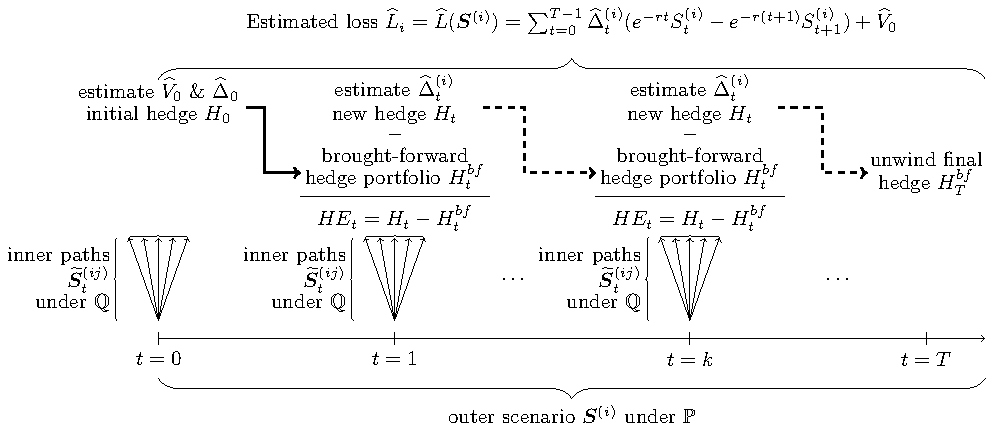
\includegraphics[width=0.85\textwidth]{./project2/figures/sns.pdf}
    \caption{Illustration of a multi-period nested simulation that estimates the P\&L for one outer scenario.}
    \label{fig2:illustration}
\end{figure}

Insurers commonly use dynamic hedging to mitigate a market risk exposure in \gls{va} contract's embedded options.
In a dynamic hedging program, a hedge portfolio is set up and periodically rebalanced for a portfolio of \gls{va} contracts using stocks, bonds, futures, and other derivatives.
For simplicity, in this study we consider delta hedging for a generic \gls{va} liability using one stock and one bond.
The metamodeling procedures presented in Section~\ref{sec2:metamodel2Stage} and Section~\ref{sec2:metamodel1Stage} can be trivially adapted to more general hedging strategies.

Consider hedging a \gls{va} contract whose sub-account is invested in a stock, and the hedging portfolio is rebalanced monthly.
At $t \leq T$, a dynamic equation can be specified for the sub-account value $F_t$, in the absence of withdrawals, as:
\begin{equation*}
    F_t = F_{t-1} \cdot \frac{S_t}{S_{t-1}} \cdot (1-\eta_g)
\end{equation*}
where $\eta_g> \eta_n$ is the gross rate of management fee that is deducted from the sub-account value at the end of each month.
The delta hedge portfolio at any month~$t$, $t=0,1,\ldots,T-1$, consists of $\Delta_t$ units in the underlying stock and $B_t$ amount of a risk-free zero-coupon bond maturing at $T$ months.
The value of the hedge portfolio at month~$(t-1)$ is:
\begin{equation*}
    H_{t-1} = \Delta_{t-1} S_{t-1} + B_{t-1},
\end{equation*}
where $S_t$ is an underlying stock price and any month $t>0$.
Assuming there is no rebalacing between $t-1$ and $t$, this hedge portfolio is brought forward to month~$t$,.
Its value at month~$t$ becomes:
\begin{equation*}
    H_{t}^{bf} = \Delta_{t-1} S_{t} + B_{t-1}e^{-rt}.
\end{equation*}
Therefore, the time~$t$ hedging error, which is the cash flow incurred by the insurer due to rebalancing at time~$t$, is
\begin{equation}\label{eq2:hedgingerror}
    HE_t = H_t - H^{bf}_t, \quad t=1,\ldots, T-1.
\end{equation}
The \gls{pl} of the \gls{va} contract includes cost of the initial hedge ($H_0$), hedging errors~\eqref{eq2:hedgingerror}, unwinding of the hedge at maturity ($H^{bf}_T$), and unhedged liability ($V_0$).
Mathematically, the present value of these cash flows is given by
\begin{equation}\label{eq2:lossrv}
L = H_0 + \sum_{t=1}^{T-1} e^{-rt} HE_t - e^{-rT} H^{bf}_T + V_0 = \sum_{t=0}^{T-1}\Delta_t (e^{-rt}S_t - e^{-r(t+1)}S_{t+1}) + V_0,
\end{equation}
where the second equality holds by a telescopic sum simplification of $e^{-rt}B_t$, $t=0,\ldots,T-1$.

In~\eqref{eq2:lossrv}, $\Delta_t$ and $V_0$ are determined by using a risk-neutral measure $\mathbb{Q}$ while the distribution of $L$ is under a real-world measure $\mathbb{P}$.
If $\Delta_t$ and $V_0$ cannot be calculated analytically, a nested simulation is required to estimate the tail risk measure of $L$.
Recall from Section~\ref{subsec:VApayout} that the stock sample path, regardless of the inner or outer simulation or a combination of both, determines the evolution of the triplet $(S_t,F_t,G_t)$.
Specifically, the outer scenarios $\bS^{(i)} = (S_{1}^{(i)},\ldots,S_{T}^{(i)})$, $i=1,\ldots,M$ are generated under $\mathbb{P}$.
At each time~$t=1,\ldots,T-1$ of a given outer scenario $\bS^{(i)}$, inner sample paths $\bStilde_{t}^{(j)} = (\Stilde_{t+1}^{(j)},\ldots,\Stilde_{T}^{(j)})$, $j=1,\ldots,N$ are generated under $\mathbb{Q}$ to estimate $\Delta_t^{(i)}$, $i=1,\ldots,M$.
Also, $V_0^{(i)}$, $i=1,\ldots,M$ are estimated under $\mathbb{Q}$ via inner simulations at time $0$.
Recall from Section~\ref{subsec:VApayout} that the stock's sample path, regardless of inner or outer simulation or a combination of both, determines the evolution of the triplet $(S_t,F_t,G_t)$.
For \gls{gmwb}, a standard nested simulation procedure to estimate the $\alpha$-\gls{cvar} of $L$ is described in Algorithm~\ref{alg2:standardProcedure} below.

\begin{algorithm} 
\caption{Standard Nested Simulation Procedure for Estimating CVaR for GMWB Hedging Losses}
\begin{algorithmic}[1] \label{alg2:standardProcedure}
    \STATE  For $i=1,\ldots,M$, simulate outer scenarios $\bS^{(i)} = (S_{1}^{(i)},\ldots,S_{T}^{(i)})$ under the real-world measure $\mathbb{P}$.
    \STATE  For $t=0$, simulate time-$0$ inner paths $\bStilde_{0}^{(j)} = (\Stilde_{1}^{(j)},\Stilde_{2}^{(j)},\ldots,\Stilde_{T}^{(j)})$, $j=1,\ldots,N$ under $\mathbb{Q}$, then estimate $V_0$ by $\Vhat_0 = \sum_{s=1}^{T} e^{-r(T-s)} [(I_s - F_s)^+- \eta_n F_s]$ and $\Deltahat_0 = \Delta_0(\Stilde_{1}^{(j)},\ldots,\Stilde_{T}^{(j)} | S_0)$.
    \STATE  Given each scenario $\bS^{(i)}$:
    \begin{enumerate}[label=\alph*., itemsep=0pt, parsep=0pt, topsep=0pt]
        \item   At each time~$t=1,\ldots,T-1$, simulate inner paths $\bStilde_{t}^{(ij)} = (\Stilde_{t+1}^{(ij)},\ldots,\Stilde_{T}^{(ij)})$, $j=1,\ldots,N$ under $\mathbb{Q}$, then estimate $\Delta_t$ by $\Deltahat_t^{(i)} = \Delta_t(\Stilde_{t+1}^{(ij)},\ldots,\Stilde_{T}^{(ij)} | \bm{S}_t^{(i)})$.
        \item   Use scenarios $\bS^{(i)}$ and $\Vhat_0$ and $\Deltahat_t^{(i)}$ to calculate losses $\Lhat_i^{MC}$, $t=0,\ldots,T-1$, then sort them as $\Lhat^{MC}_{(1)}\leq \Lhat^{MC}_{(2)} \leq \cdots\leq \Lhat^{MC}_{(M)}$.
    \end{enumerate}
    \STATE  Estimate $\alpha$-CVaR of $L$ by $\widehat{\CVaR}^{MC}_\alpha = \frac{1}{(1-\alpha)M} \sum_{i=\alpha M + 1}^{M}\Lhat_{(i)}^{MC} = \frac{1}{(1-\alpha)M} \sum_{i \in \widehat{\tail}_{(1-\alpha )M}^{MC}}\Lhat_{i}^{MC}$.
\end{algorithmic}
\end{algorithm}

We refer to the collection of experiments needed conditional on one scenario $\bS^{(i)}$ to estimate $L_i$, which is all upward arrows in Figure~\ref{fig2:illustration}, as one inner simulation.
We make four observations:
\begin{itemize}
    \item   Each inner simulation is time-consuming, as it includes $T$ simulation experiments: one at each time $t=0,\ldots,T-1$,
    \item   After running inner simulations for $M$ scenarios, we obtain simulated data as feature-label pairs, $(\bS^{(i)}, \Lhat_i)$, $i=1,\ldots,M$; the feature vector $\bS$ is $T$ dimensional.
    \item   $\Lhat_i^{MC}$ is a standard Monte Carlo estimator of the true loss for scenario $\bS^{(i)}$. 
    It is an unbiased estimator and its variance is inversely proportional to the number of inner replications $N$. 
    As $N$ approaches infinity, $\Lhat_i^{MC}$ converges to the true loss $L_i$, and
    \item   Most importantly, when estimating tail risk measures such as $\alpha$-\gls{cvar}, only a small number of estimated losses, which is those associated with the set of tail scenarios $\widehat{\tail}_{k}$ are used in the estimator.
\end{itemize}

\section{Two-Stage Nested Simulation with Metamodels} \label{sec2:metamodel2Stage}

Based on the three observations above and built on the work by~\cite{dang2020efficient}, we propose a two-stage nested simulation procedure which uses a \gls{dnn} metamodel to identify potential tail scenarios.
We present our proposed procedure as a competitor to the standard procedure with $M$ outer scenarios and $N$ inner replications for each outer scenario, as described in Section~\ref{subsec:dynamicHedge}.
We propose a two-stage procedure with a supervised learning metamodel that aims at producing a \gls{cvar} estimate that is as accurate as that of the standard procedure, but requires fewer computations than the latter.

\begin{algorithm}
\caption{Two-Stage Metamodeling Nested Simulation Procedure for Estimating CVaR}
\begin{algorithmic}[1] \label{alg2:twoStageProcedure}
    \STATE \textbf{Train a neural network metamodel using simulation data:}
    \begin{enumerate} [label=\alph*., itemsep=0pt, parsep=0pt, topsep=0pt]
        \item Use a fraction of the total simulation budget to run Steps 1, 2, and 3 in the standard procedure, i.e., Algorithm~\ref{alg2:standardProcedure}, with the same number of outer scenarios, $M$, but a much smaller number of inner replications, $N' \ll N$, in each scenario. 
        Obtain $M$ simulated samples (feature-label pairs), $(\bS^{(i)}, \Lhat_i)$, $i=1,\ldots,M$. 
        Note that $N'$ may be much smaller than $N$, so $\Lhat_i$ are expected to have larger variance.
        \item Use the simulated data, $(\bS^{(i)}, \Lhat_i)$, $i=1,\ldots,M$ to train a supervised learning model. 
        It is standard practice in supervised learning research to transform the stock prices $\bS^{(i)}$ to returns $\mathbf{X}^{(i)}$,
        \begin{equation} \label{eq2:return}
        \mathbf{X}^{(i)} = \left(\frac{S_1^{(i)} - S_0}{S_0}, \frac{S_2^{(i)} - S_1^{(i)}}{S_1^{(i)}}, \ldots, \frac{S_T^{(i)} - S_{T-1}^{(i)}}{S_{T-1}^{(i)}}\right)
        \end{equation}
        and use $\mathbf{X}^{(i)}$ as features instead of the stock prices $\bS^{(i)}$.
        Refer to the trained model as a metamodel and denote it by $\Lhat^{PD}(\mathbf{X})$. Denote the predicted losses for the outer scenarios by $\Lhat^{PD}_i = \Lhat^{PD}(\mathbf{X}^{(i)})$, $i=1,\ldots,M$.
        \item Sort the predicted losses $\Lhat^{PD}_{(1)}\leq \Lhat^{PD}_{(2)} \leq \cdots\leq \Lhat^{PD}_{(M)}$ to identify a predicted tail scenario set, $\widehat{\tail}_{m}^{PD}$, associated with the largest predicted losses. The number of predicted tail scenarios, $m$, is a user's choice.
    \end{enumerate}
    \STATE \textbf{Concentrate simulation on predicted tail scenarios:}
    \begin{enumerate} [label=\alph*., itemsep=0pt, parsep=0pt, topsep=0pt]
        \item Run Steps 2 and 3 of Algorithm~\ref{alg2:standardProcedure} with the same number of inner replications, $N$, but only on the predicted tail scenarios, i.e., scenarios in $\widehat{\tail}_{m}^{PD}$. Denote the standard procedure's estimated losses and sorted losses by $\Lhat^{ML}_i$ and $\Lhat^{ML}_{(i)}$, respectively, $i=1,\ldots,m$.
        \item Estimate the $\alpha$-CVaR of $L$ by 
        $$\widehat{\CVaR}^{ML}_\alpha = \frac{1}{(1-\alpha)M} \sum_{i=\alpha M + 1}^{M}\Lhat_{(i)}^{ML} = \frac{1}{(1-\alpha)M} \sum_{i \in \widehat{\tail}_{(1-\alpha)M}^{ML}}\Lhat_{i}^{ML},$$ 
        where $\widehat{\tail}_{k}^{ML}$ denotes a predicted tail scenario set associated with the largest $k$ estimated losses.
    \end{enumerate}
\end{algorithmic}
\end{algorithm}

Similar to~\cite{dang2020efficient}, the proposed two-stage procedure in Algorithm~\ref{alg2:twoStageProcedure} uses the metamodel predictions to identify the predicted tail scenario set in stage 1.
However, different from their fixed-budget simulation design, we attempt to achieve a target accuracy.
Specifically, in stage 2 we propose using a standard procedure with the same number of inner replications, $N$, as a benchmark procedure.
There are two different types of experiment designs for nested simulation procedures: fixed-budget design and fixed-accuracy design.
In a fixed-budget design, the simulation budget is fixed, and the goal is to achieve the highest degree of accuracy possible within the budget.
Let $\Gamma = MN$ be the simulation budget for the standard procedure, where each scenario receives $\frac{\Gamma}{M}$ inner replications.
In the proposed two-stage procedure, suppose that stage 1 uses $1\%$ of the simulation budget, $\alpha = 95\%$, and $m=(1-\alpha)M$, then $99\%$ of the simulation budget is concentrated on $5\% M$ predicted tail scenarios in stage 2.
In other words, each predicted tail scenario receives $\frac{99\% \Gamma}{5\% M}$ inner replications, almost 20 times more than that in the standard procedure.
This budget concentration is expected to improve the estimation accuracy of the two-stage procedure compared to a standard procedure with the same budget. 
If the metamodel is accurate in predicting true tail scenarios, the two-stage procedure is expected to achieve a higher degree of accuracy than the standard procedure with the same budget.
However, we believe that the goal of designing an efficient simulation procedure is to solve practical problems faster, so a target-accuracy design is more suitable, which refers to obtaining a similar level of accuracy as the standard procedure but with much less simulation budget.
One other reason for recommending this fixed-accuracy design is to investigate whether \gls{dnn} metamodels trained with much noisier labels can identify true tail scenarios with a similar degree of accuracy as the standard procedure.
The size of the predicted tail scenario set in stage 1, $m$, is an important experiment design parameter that affects the correct identification of true tail scenarios and ultimately affects the estimation accuracy for \gls{cvar}.
Clearly, there is a lower bound $m \geq (1-\alpha)M$ because the $\alpha$-\gls{cvar} is estimated by the average of the largest $(1-\alpha)M$ losses at the end of stage 2.
For ease of reference, we call the additional percentage of predicted tail scenarios above this lower bound, i.e., $\epsilon = \frac{m - (1-\alpha)M}{M}$, as a \textit{safety margin}.
On one hand, large $\epsilon$ is not desirable because it increases computations in stage 2.
On the other hand, $\epsilon$ should be set reasonably large so that more true tail scenarios are included in the predicted tail scenario set $\widehat{\tail}_{m}^{PD}$ and are ultimately included in $\widehat{\tail}_{(1-\alpha )M}$ at the end of stage 2.
The selection of $m$ is highly dependent on the choice of the metamodel.
Due to the simulation errors and approximation error in the metamodel in stage 1, we do not expect a perfect match between the true tail scenario set $\tail_{k}$ and the predicted tail scenario set $\widehat{\tail}_{k}^{PD}$ for any size $k$.
This means that we should not set $m$ at its lower bound: Some safety margin $\epsilon M$ should be added to the predicted tail scenario set, i.e., $m = (1-\alpha )M + \epsilon M$, to increase the likelihood that $\tail_{k} \subseteq \widehat{\tail}_{m}^{PD}$ and that the true tail scenarios are included in estimating $\alpha$-\gls{cvar} at the end of stage 2.
The choice of a safety margin $\epsilon$ is not trivial, and it should be set based on the metamodel's accuracy in identifying true tail scenarios.
In the numerical experiments, we examine the relationship between the safety margin and the correct identification of true tail scenarios for different metamodels.

\section{Single-Stage Nested Simulation with Neural Network Metamodels} \label{sec2:metamodel1Stage}

In our exploratory experiment with the two-stage procedure, we observe that a suitable metamodel trained with noisy labels is accurate enough to identify true tail scenarios with a relatively small safety margin.
This observation motivates us to propose a single-stage procedure that uses the identical neural network metamodel, not for the purpose of differentiating between tail and non-tail scenarios, but rater to estimate the \gls{cvar} directly using the predicted losses. 

\begin{algorithm}
\caption{Single-Stage Metamodeling Nested Simulation Procedure for Estimating CVaR}
\begin{algorithmic}[1] \label{alg2:oneStageProcedure}
    \STATE Run Step 1 of Algorithm~\ref{alg2:twoStageProcedure}, and denote the predicted losses by
    $\Lhat^{PD}_i = \Lhat^{PD}(\bS^{(i)})$, $i=1,\ldots,M$.
    \STATE Sort the predicted losses $\Lhat^{PD}_{(1)}\leq \Lhat^{PD}_{(2)} \leq \cdots\leq \Lhat^{PD}_{(M)}$ to identify the largest predicted losses. 
    \STATE Directly estimate the risk measure (e.g., $\alpha$-CVaR) of $L$ using the metamodel predictions: Calculate $\widehat{\CVaR}^{PD}_\alpha = \frac{1}{(1-\alpha)M} \sum_{i=\alpha M + 1}^{M}\Lhat^{PD}_{(i)}$.
\end{algorithmic}
\end{algorithm}

The single-stage procedure has three major advantages over the two-stage procedure:
\begin{enumerate}
    \item The single-stage procedure is expected to be more efficient than the two-stage procedure because it does not require us to run the standard procedure described in stage 2.
    \item The safety margin $\epsilon$ is not needed in the single-stage procedure.
    The safety margin is difficult to determine because it depends on the metamodel's accuracy in identifying true tail scenarios.
    The single-stage procedure does not need a safety margin because it directly estimates the risk measure by using the predicted losses.
    \item Most importantly, the single-stage procedure is not limited to just estimating tail risk measures and can be extended to provide a broader assessment of risk. 
    It can be naturally adapted to estimate risk measures that require the knowledge of the entire loss distribution, such as the standard deviation or the squared tracking error.
    Even for \gls{cvar}, the two-stage procedure becomes less attractive at a higher level of $\alpha$.
\end{enumerate}

\section{Numerical Results} \label{sec2:numerical}

We conduct a series of simulation experiments to 
\begin{enumerate}
    \item demonstrate the efficiency of the proposed metamodeling procedures, and
    \item examine the error tolerance to noisy training data in deep learning models.
\end{enumerate}
The problem settings in our experiments are identical to those in~\cite{dang2020efficient}.
We consider estimating the $95\%$ \gls{cvar} of the hedging loss of a \gls{gmwb} contract, which is one of the most complex \gls{va} contracts in the market.
The \gls{va} contracts have a 20-year maturity and are delta-hedged with monthly rebalancing, i.e., $T=240$ rebalancing periods.
The gross and net management fees are $\eta_g = 0.2\%$ and $\eta_n=0.1\%$, respectively.
The withdrawal rate for \gls{gmwb} is $0.375\%$ per month.
To make our examples more realistic, the \gls{va}s are also subject to a dynamic lapse model with the following key features~\citep{naic2021}:
\begin{enumerate}
    \item When a policyholder lapses, both the fund value ($F$) and guarantee value ($G$) are reduced proportionally.
    \item The monthly lapse rate from time $t$ to $t + 1$, denoted as ${}_{\frac{1}{12}}q^l_{x+\frac{t}{12}}$, is given by:
    \begin{equation} \label{eq:dynamic_lapse_rate}
        {}_{\frac{1}{12}}q^l_{x+\frac{t}{12}} = \min\left\{1, \max\left\{0.5, 1 - 1.25 \times \left(\frac{G_t}{F_t} - 1.1\right)\right\} \times {}_{\frac{1}{12}}q^{base}_{x+\frac{t}{12}}\right\}
    \end{equation}
    where ${}_{\frac{1}{12}}q^{base}_{x+\frac{t}{12}}$ is a base monthly mortality rate for a policyholder aged $x + \frac{t}{12}$ at month $t$, and the base monthly lapse rate is defined as:
    \begin{equation} \label{eq:lapse_rate}
        {}_{\frac{1}{12}}q^{base}_{x+\frac{t}{12}} = 
        \begin{cases}
            0.00417 & \text{if } t < 84, \\
            0.00833 & \text{if } t \geq 84.
        \end{cases}
    \end{equation}
\end{enumerate}

The risk-free rate is $0.2\%$ per month and the underlying asset $S_t$ is modeled by a regime-switching geometric Brownian motion with parameters specified in Table~\ref{tab:regime_params}.

\begin{table}[ht]
    \centering
    \begin{tabular}{lc}
        \toprule
        \textbf{Parameter}  & \textbf{Monthly Value} \\
        \midrule
        Risk-free rate & $0.002$ \\
        Mean return for regime 1  & $0.0085$ \\
        Mean return for regime 2   & $-0.0200$ \\
        Standard deviation for regime 1  & $0.035$ \\
        Standard deviation for regime 2  & $0.080$ \\
        Transition probability from regime 1  & $0.04$ \\
        Transition probability from regime 2  & $0.20$ \\
        \bottomrule
    \end{tabular}
    \caption{Real-world parameters for the regime-switching model (monthly rates)}
    \label{tab:regime_params}
\end{table}

To compare the numerical performances of different simulation procedures, we create a benchmark dataset with a large-scale nested simulation: We first simulate $M=\num{100000}$ outer scenarios, i.e., $240$-periods stock paths $\bS^{(1)},\ldots,\bS^{(M)}$ under $\mathbb{P}$ and used these outer scenarios in all further experiments.
Note that the $5\%$ tail scenario set includes $\num{5000}$ scenarios.
As the hedging losses for these scenarios cannot be calculated analytically, we run inner simulations with a large number of replications, $N=\num{100000}$, conditional on each of the $M$ scenarios.
We denote these losses by $L_1,\ldots,L_M$ and will refer to them as \textit{true losses}.
We also use these true losses to estimate $\widehat{\CVaR}_{95\%}$ and denote the corresponding \textit{true tail scenario set} by $\tail_{5000}$.
Lastly, we refer to the set of feature-label pairs $\{(\bS^{(i)}, L_i): i=1,\ldots,M\}$ as a \textit{true dataset}.
Note that the feature vector $\bS$ is a 240-dimension stock path.

In our experiments, the standard nested simulation procedure is mainly used in three ways.
\begin{enumerate}
    \item   The true losses and the true $95\%$-\gls{cvar} are estimated by using a standard nested simulation procedure that runs $N=\num{100000}$ inner replications for each of the $M=\num{100000}$ outer scenarios.
    \item   A benchmark estimator of the $95\%$-\gls{cvar} is generated by using $N=\num{1000}$ for each of the $M=\num{100000}$ outer scenarios.
    \item   The training data for our metamodels is generated by using $N=\num{100}$ for $M=\num{100000}$.
    The value of $M$ and $N$ are subject to change in our other numerical experiments.
\end{enumerate}

Five metamodels are considered in this experiment: \gls{mlr}, \gls{qpr} without interaction terms, \gls{fnn}, \gls{rnn}, and \gls{lstm} network.
\gls{mlr} and \gls{qpr} are two common metamodels in the simulation literature, and their implemention is straightfoward in our simulation setting.
\gls{fnn} is a generic neural network while \gls{rnn} and \gls{lstm} are specialized models to accommodate the sequential structure of our time-series features.
A $\tanh$ activation function is used for \gls{rnn} and \gls{lstm} layers, and a ReLU activation function is used for the fully-connected layers.
All neural network metamodels are trained by the Adam optimizer~\citep{kingma2014adam} with an initial learning rate of $0.001$ and an exponential learning rate decay schedule.
All \gls{dnn} metamodels are trained with a dropout rate of $10\%$.
The architectures and training settings are typical choices in the deep learning literature.
The training labels are normalized to have a zero mean and a unit standard deviation.
The numbers of trainable parameters are recorded in the second column of Table~\ref{tab:gmwb_arch}.
We observe that the three \gls{dnn} metamodels have orders of magnitudes more trainable parameters than the two traditional regression metamodels.
Following the convention in machine learning literature, the three \gls{dnn} metamodels are said to have much higher \textit{model capacities}.
Treating regression metamodels as shallow neural networks, \gls{mlr} and \gls{qpr} are two neural networks with no hidden layer. 
For a traditional regression metamodel, the numbers of neurons in its input layer equals to the cardinality of its regression basis.
On the other hand, the three \gls{dnn} metamodels have several hidden layers and are more flexible than \gls{mlr} and \gls{qpr}.
Our \gls{fnn} has two hidden layers prior to its output layer.
Its hidden layers are feature extraction layers that transform the 240-dimension feature vector into a 32-dimension vector that can directly relate to the target variable.
This extraction process is automatic and does not require manual feature engineering.
Our \gls{rnn} and \gls{lstm} networks have three hidden layers.
They contain similar numbers of neurons as the \gls{fnn} but have deeper network structures.
For \gls{rnn}, two of its hidden layers are recurrent layers that capture the temporal dependency in the feature, and its last hidden layer is a standard feedforward layer that transforms the previous hidden states into a 32-dimension vector for target prediction.
Our \gls{lstm} has the same architecture as the \gls{rnn} but with \gls{lstm} cells in place of \gls{rnn} cells.

% Fill this table with new results
\begin{table}[ht!]
    \centering
    \footnotesize
    \begin{tabular}{lcccc}
    \toprule
    \textbf{Metamodel} & \textbf{\makecell{Capacity}} & \textbf{Training error} & \textbf{Test error} & \textbf{True error}\\
    \midrule
    \gls{mlr} & $\num{241}$ & $0.706 (\pm 8.34\times 10^{-4})$ & $0.713 (\pm 2.67 \times 10^{-2})$ & $0.706 (\pm 3.44 \times 10^{-4})$ \\
    \gls{qpr} & $\num{481}$ & $0.543 (\pm 8.27\times 10^{-4})$ & $0.554 (\pm 2.32 \times 10^{-2})$ & $0.544 (\pm 4.12\times 10^{-4})$ \\
    \gls{fnn} & $\num{35009}$ & $0.129 (\pm 5.95\times 10^{-3})$ & $0.240 (\pm 9.82 \times 10^{-3})$ & $0.132 (\pm 5.82\times 10^{-3})$ \\
    \gls{rnn} & $\num{32021}$ & $0.132 (\pm 7.53\times 10^{-3})$ & $0.137 (\pm 7.62\times 10^{-3})$ & $0.119 (\pm 7.51\times 10^{-3})$ \\
    \gls{lstm} & $\num{35729}$ & $0.075 (\pm 4.48\times 10^{-3})$  & $0.079 (\pm 5.35\times 10^{-3})$ & $0.063 (\pm 4.43\times 10^{-3})$ \\
    \gls{rnn}$^*$\footnotemark & $\num{32021}$ & $0.109 (\pm 5.20\times 10^{-3})$  & $0.128 (\pm 5.22\times 10^{-3})$  & $0.109 (\pm 5.20\times 10^{-3})$ \\
    \bottomrule
    \end{tabular}
    \caption{Architectures and \gls{mse}s of metamodels for \gls{gmwb} inner simulation model.}
    \label{tab:gmwb_arch}
\end{table}

\footnotetext{This row summarizes the error metrics of the well-trained \gls{rnn}, where the ones suffer from a vanishing gradient issue are removed from the averages.}

For each metamodel, \num{100} independent macro replications are run.
Each macro replication involves simulating a noisy dataset, randomly separating it into training and test data, fitting a metamodel, and forming predictions.
The last three columns in Table~\ref{tab:gmwb_arch} display the average squared errors between the metamodel predictions and the loss labels for different datasets.
Training error, test error, and true error are the average squared errors between the metamodel predictions and the training labels, test labels, and true labels, respectively.
The half lengths of their $95\%$ confidence bands are also reported in parentheses.
We first observe that the two regression metamodels have high training errors.
This is a sign of under-fitting.
Model capacities of the regression metamodels are too low to learn the training dataset.
A successful learning on the training dataset is a necessary condition for a metamodel to generalize to the true simulation model.
All neural network metamodels have high model capcities comparing with the number of data points in the training set, i.e., $\num{90000}$.
Empirically, this is not a huge concern for the \gls{dnn}s.
In neural network literature, the number of trainable parameters is often much larger than the number of training samples.
AlexNet~\citep{krizhevsky2012imagenet}, a well-known CNN, has $\num{60}$ million trained parameters and is trained on the ImageNet dataset with only $1.2$ million sample images.
Other examples include generative pre-trained transformer models like BERT~\citep{devlin2018bert} and GPT-3~\citep{brown2020language}, which have billions of trainable parameters and are trained on large-scale text corpora.
The reason for not over-fitting when the number of trainable parameters is much larger than the number of training samples is still an open question in deep learning community.
One of the explanations in the literature is that the optimization surface of \gls{dnn}s is highly non-convex and has many local minima.
Given a good initialization, the optimization algorithm is likely to find a solution that generalizes well to unseen data.
Another explanation is that most existing \gls{dnn} models have specific architectures that make them less prone to over-fitting.
For example, a \gls{cnn} is specifically designed to capture a spatial structure in image data.
Unlike the \gls{fnn}, not all neurons are connected to all neurons in the previous layer.
This architecture serves as prior knowledge and a form of regularization that make \gls{cnn}s less prone to over-fitting.

In our experiments, there are important differences among the three \gls{dnn} models due to having different neural network architectures.
Their model capacities are intentionally set to be similar to each other for a fair comparison.
The \gls{fnn} is a generic neural network, its test error is much greater than the training error, which is a sign of over-fitting and poor generalization.
In contrast, \gls{rnn} and \gls{lstm} networks have recurrent structures and are designed to capture temporal relationship in the high-dimensional feature.
As a result, they have lower training errors.
They fit the data better and have lower test errors, i.e., they generalize better.
Notably, the true errors for the \gls{dnn} metamodels are lower than the training errors.
This is a sign of the metamodels' ability to learn the true feature-label relationship with noisy training labels. 
Section~\ref{subsec2:noiseTolerance} investigates this phenomenon in greater details.

The intuition behind the \gls{rnn} and \gls{lstm} metamodels is briefly mentioned in~\ref{subsec:LSTM}.
To overcome the overfitting issue of the \gls{fnn}, \gls{rnn} learns a single function that operates across all time steps, and the time $t$ itself is not a variable in the \gls{rnn}.
The \gls{rnn} cells in \gls{rnn} and \gls{lstm} networks share parameters across time and serve as a form of regularization that prevents overfitting.
However, the price that \gls{rnn} pays for a reduced number of parameters is the difficulty in its optimization.
Comparing the two metamodels with recurrent structures, a \gls{lstm} network overcomes two key drawbacks of a crude \gls{rnn}.
\begin{enumerate}
    \item It avoids the vanishing gradient problem during training, which makes the \gls{lstm} network easier to train than the \gls{rnn}. Figure~\ref{fig2:QQ_RNN} shows the quantile-quantile (QQ) plots between the \textbf{training} labels and the \gls{rnn} predictions for two macro replications, where training of the latter is hindered by the vanishing gradient problem. 
    As a result, the half-width of the $95\%$ confidence band of the \gls{rnn}'s training error is much larger than all other metamodels. 
    The last row of Table~\ref{tab:gmwb_arch} shows the average squared errors of the good \gls{rnn} metamodels that have been successfully trained. 
    Removing the \gls{rnn} metamodels that are ill-trained, the average squared errors of the \gls{rnn} metamodels are lower than those of the \gls{fnn}.
    This suggests that the \gls{rnn} is more sensitive to noise in the sense of a stochastic gradient descent than the \gls{fnn}.
    They can capture the temporal dependency but are more difficult to optimize.
    \item A \gls{lstm} introduces three gates that regulate the flow of information. 
    These gates decide what information should be kept or discarded.
    For detailed discussion on the \gls{lstm} network, please refer to Section~\ref{subsec:LSTM}.
    This gating mechanism makes a \gls{lstm} network more capable of learning long-term dependencies. 
    Since the feature in our dynamic hedging problem is a 240-dimensional time series, a \gls{lstm} network is more suitable than a crude \gls{rnn}.
\end{enumerate}
In summary, the network depth ensures successful learning of the training dataset, and the network architecture serves as 
The intuition behind the \gls{rnn} and \gls{lstm} metamodels is briefly mentioned in~\ref{subsec:LSTM}.
To overcome the overfitting issue of the \gls{fnn}, \gls{rnn} learns a single function that operates across all time steps, and the time $t$ itself is not a variable in the \gls{rnn}.
The \gls{rnn} cells in \gls{rnn} and \gls{lstm} networks share parameters across time and serve as a form of regularization that prevents overfitting.
However, the price that \gls{rnn} pays for a reduced number of parameters is the difficulty in its optimization.
Comparing the two metamodels with recurrent structures, a \gls{lstm} network overcomes two key drawbacks of a crude \gls{rnn}.
\begin{enumerate}
    \item It avoids the vanishing gradient problem during training, which makes the \gls{lstm} network easier to train than the \gls{rnn}. Figure~\ref{fig2:QQ_RNN} shows the quantile-quantile (QQ) plots between the \textbf{training} labels and the \gls{rnn} predictions for two macro replications, where training of the latter is hindered by the vanishing gradient problem. 
    As a result, the half-width of the $95\%$ confidence band of the \gls{rnn}'s training error is much larger than all other metamodels. 
    The last row of Table~\ref{tab:gmwb_arch} shows the average squared errors of the good \gls{rnn} metamodels that have been successfully trained. 
    Removing the \gls{rnn} metamodels that are ill-trained, the average squared errors of the \gls{rnn} metamodels are lower than those of the \gls{fnn}.
    This suggests that the \gls{rnn} is more sensitive to noise in the sense of a stochastic gradient descent than the \gls{fnn}.
    They can capture the temporal dependency but are more difficult to optimize.
    \item A \gls{lstm} introduces three gates that regulate the flow of information. 
    These gates decide what information should be kept or discarded.
    For detailed discussion on the \gls{lstm} network, please refer to Section~\ref{subsec:LSTM}.
    This gating mechanism makes a \gls{lstm} network more capable of learning long-term dependencies. 
    Since the feature in our dynamic hedging problem is a 240-dimensional time series, a \gls{lstm} network is more suitable than a crude \gls{rnn}.
\end{enumerate}
In summary, the network depth ensures successful learning of the training dataset, and the network architecture serves as 
\begin{enumerate}
    \item regularization that prevents over-fitting, and 
    \item prior knowledge that guides the optimization algorithm to find a solution that generalizes well to unseen data.
\end{enumerate}
They are both crucial for the metamodels' performance.
It is important to choose a \textit{suitable} architecture with a pre-set capacity that is large enough to learn the training dataset and generalize to the true feature-label relationship.

\begin{figure}[ht!]
    \centering
    \begin{subfigure}{0.48\textwidth}
        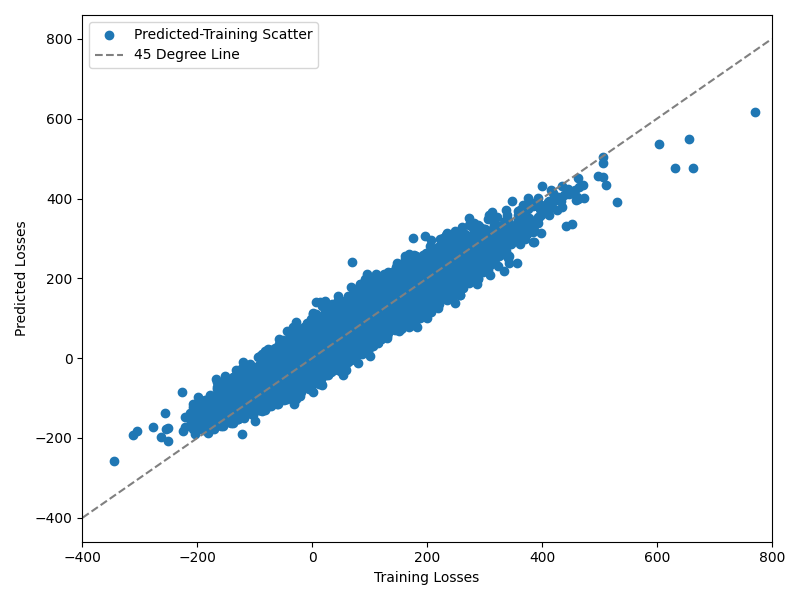
\includegraphics[width=\textwidth]{./project2/figures/2a_QQ_good_training.png}
        \caption{A good RNN metamodel}
    \end{subfigure}\hfill
    \begin{subfigure}{0.48\textwidth}
        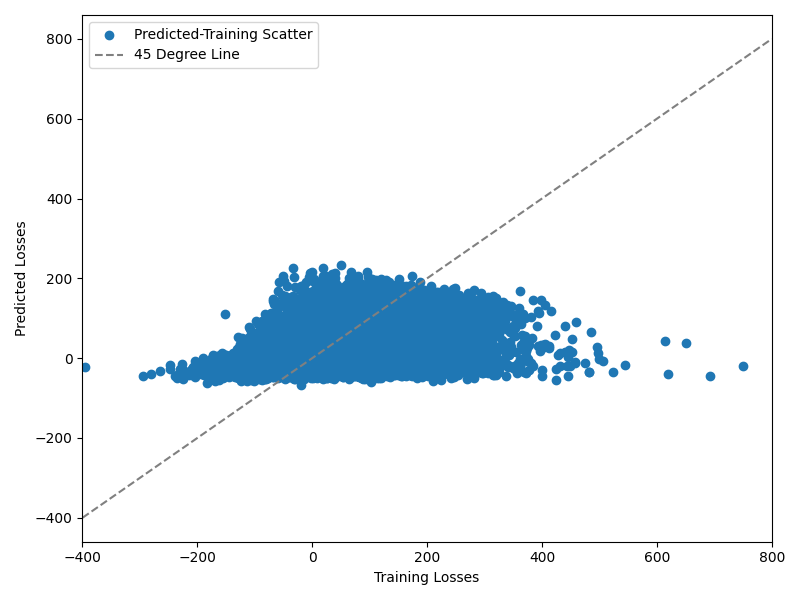
\includegraphics[width=\textwidth]{./project2/figures/2b_QQ_bad_training.png}
        \caption{A bad RNN metamodel}
        \label{subfig2:badRNN}
    \end{subfigure}
    \caption{QQ-plots between true labels (x-axis) and predicted losses (y-axis) for the RNN metamodel.} 
    \label{fig2:QQ_RNN}
\end{figure}

Recall that all three datasets are generated from the same simulation model, but the true labels contain much less simulation noise than the training and test labels.
Part of the training error is from the simulation noise, and this noise is much less reflected in the true error.
We observe that the two regression metamodels is under-fitting with high training errors. 
They also have low test and true errors, which indicates poor generalization.
In contrast, the \gls{dnn} metamodels have lower errors.
More specifically, they generalize better to the true labels than to the test labels.
The test labels contain more simulation noise than the true labels.
This is a sign of the regression metamodels' inability to learn the true feature-label relationship rather than merely over-fitting to the simulation noise in the training labels.
In practical applications, the true labels are not available.
However, analyzing the quality of fit on the true labels in a simulation environment offers a unique opportunity to understand the metamodels' true ability of learning.
Figure~\ref{fig2:QQ_REG} and Figure~\ref{fig2:QQ_NN} shows the QQ plots between the \textbf{true} loss labels and the predicted losses for the regression metamodels and the neural network metamodels, respectively.

\begin{figure}[ht!]
    \centering
    \begin{subfigure}{0.48\textwidth}
        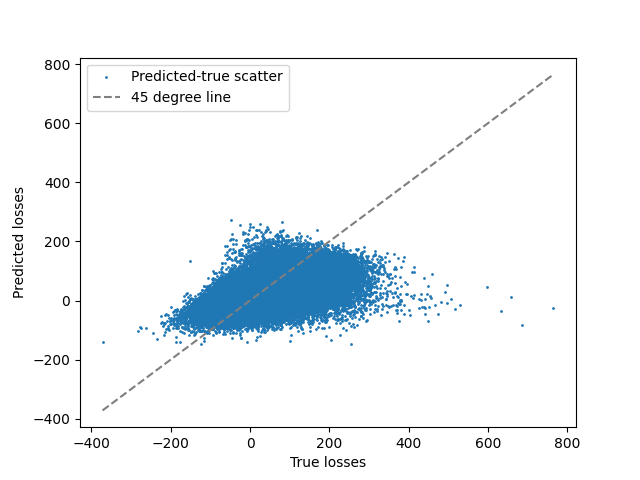
\includegraphics[width=\textwidth]{./project2/figures/qqPlots/mlrLN.png}
        \caption{MLR metamodel}
    \end{subfigure}\hfill
    \begin{subfigure}{0.48\textwidth}
        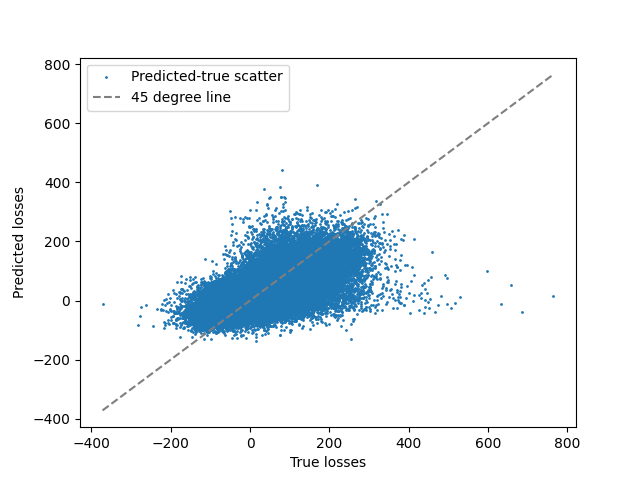
\includegraphics[width=\textwidth]{./project2/figures/qqPlots/qprLN.png}
        \caption{QPR metamodel}
    \end{subfigure}
    \caption{QQ-plots between true losses (x-axis) and predicted losses (y-axis) for regression metamodels.} 
    \label{fig2:QQ_REG}
\end{figure}

Comparing with the \gls{mse} table in Table~\ref{tab:gmwb_arch} that summarizes the overall fit, QQ plots offer a closer look at the metamodels' performance on different parts of the loss distribution.
Figure~\ref{fig2:QQ_REG} show the regression metamodel predictions and the loss labels in the true dataset.
Between the two regression metamodels, the \gls{qpr} metamodel has a slightly better fit for larger losses.
Nevertheless, the predictions of both regression metamodels are far from the true labels, and their fit on the tail is particularly undesirable.
The poor fit on the tail hinders the regression metamodels' ability to identify true tail scenarios and ultimately leads to poor \gls{cvar} estimates.
Adding the quadratic terms, our \gls{qpr} metamodel is considered as a natural extension of the \gls{mlr}.
Attempts to further improve the regression metamodels by adding interaction terms or higher-order terms do not improve the fit.
Feature engineering (i.e., variable selection) for regression metamodels is not a trivial task and is highly dependent on the simulation procedure. 
Having $240$ time-series features further complicates this issue.
As a result, our attempts to improve the traditional regression metamodels are not successful.
The regression metamodels are not flexible enough to capture the complex feature-label relationship in the dynamic hedging simulation model.

\begin{figure}[ht!]
    \centering
    \begin{subfigure}{0.48\textwidth}
        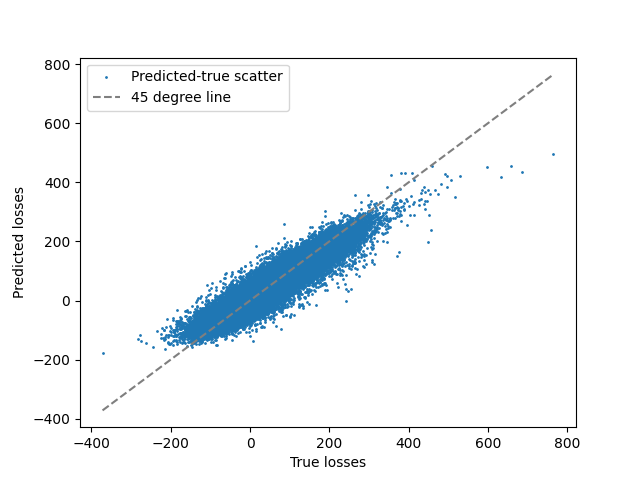
\includegraphics[width=\textwidth]{./project2/figures/qqPlots/fnnLN.png}
        \caption{FNN metamodel}
    \end{subfigure}\hfill
    \begin{subfigure}{0.48\textwidth}
        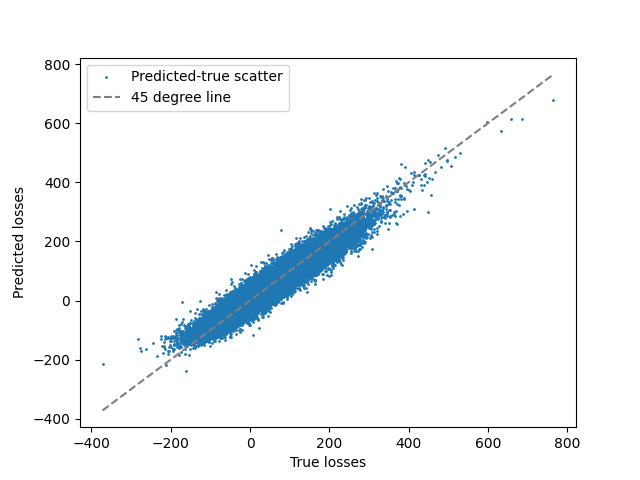
\includegraphics[width=\textwidth]{./project2/figures/qqPlots/lstmLoCapLN.png}
        \caption{LSTM metamodel}
    \end{subfigure}
    \caption{QQ-plots between true losses (x-axis) and predicted losses (y-axis) for neural network metamodels.} 
    \label{fig2:QQ_NN}
\end{figure}

In Figure~\ref{fig2:QQ_NN}, we illustrate the fit of the neural network metamodels.
The \gls{fnn} has a better fit than the regression metamodels, but it still has a poor fit on the tails.
We observe that the \gls{lstm} metamodels' QQ-plots closely follow the $45$-degree line.
Again, these metamodels are trained on noisy data, so the good fit to the true data should not be taken for granted.
This implies that these models indeed learn the true feature-label relationship in the dynamic hedging simulation model (i.e., true loss labels) even though they are trained on noisy observations (e.g., training labels) of the model.

From a unique analytical standpoint, our numerical study offers a methodical exploration into the robustness of \gls{dnn} models against noise in training labels. 
By employing the standard nested simulation procedure in Algorithm~\ref{alg2:standardProcedure} as a data generator, we gain the ability to manipulate the noise level by adjusting the number of inner replications while keeping the same simulation procedure.
This approach provides a controlled environment to examine the impact of label noise on neural network models.
It allows us to generate our true dataset that approximates the true hedging losses with a high degree of precision, and, as a result, it enables us to explore the crucial question of whether deep learning models are capable of learning the true feature-label relationship from noisy training labels.
Our numerical results in Table~\ref{tab:gmwb_arch} and the QQ plots provide direct evidence that \gls{dnn} models are indeed able to cut through the noise in the training labels and learn the true feature-label relationship.
The \gls{lstm} metamodels' ability to learn the true feature-label relationship is crucial for the two-stage procedure to identify true tail scenarios and produce accurate \gls{cvar} estimates.
Section~\ref{subsec2:noiseTolerance} discusses \gls{lstm} metamodels in more details regarding their sensitivity to data quality and quantity.
We aim at providing numerical evidence and insights into the \gls{dnn} metamodels' noise tolerance.

\subsection{Two-Stage Procedure} \label{subsec:twoStageProcedure}

We compare our two-stage procedure to a benchmark standard nested simulation procedure that runs $N=\num{1000}$ inner replications for each of the $M=\num{100000}$ outer scenarios.
In stage 1 of the proposed procedure, we first run inner simulations with $N'=100$ inner replications for each of the $M=\num{100000}$ outer scenarios.
So, stage 1's simulation budget is $10\%$ of the standard procedure's.
The resulting feature-label pairs $\{(\bS^{(i)}, \Lhat_i): i=1,\ldots,M\}$ is used for training different  metamodels.
Specifically, following the convention in machine learning literature, we split this dataset into three parts: The training, validation, and test sets have $\num{90000}$, $\num{5000}$, and $\num{5000}$ samples (representing $90\%$, $5\%$, and $5\%$ of the dataset), respectively.
At the end of stage 1, $m$ predicted tail scenarios are identified by the trained metamodels.
In stage 2, $N=\num{1000}$ inner replications are run for all predicted tail scenarios.
This is the same number of replications as the benchmark standard procedure.
Stage 2's simulation budget is $\frac{m}{M}$ of the benchmark standard procedure's.
In short, the two-stage procedure uses $15\% - 30\%$ of the benchmark procedure's budget for a safety margin between $0\% - 15\%$.
Analyzing the two stages separately, the simulation budget for stage 1 is $10\%$ of the benchmark procedure's.
Stage 2 uses $5\%$ to $20\%$ of the simulation budget of the benchmark procedure for a safety margin between $0\% - 15\%$.

In our proposed two-stage procedure, the metamodel is used to identify the predicted tail scenario set, on which the standard nested simulation procedure is run in stage 2 to estimate the $95\%$-\gls{cvar}.
An accurate identification of the true tail scenarios is crucial.
In a two-stage procedure, metamodels' overall prediction errors measured by the MSEs in Table~\ref{tab:gmwb_arch} are not the determining factor, but their ability to effectively rank the scenarios by their \textbf{true} losses is most critical in producing accurate \gls{cvar} estimates. 
A metamodel that uses less safety margin to rank can save more simulation budget in stage 2.

\begin{figure}[ht!]
    \centering
    \begin{subfigure}{0.48\textwidth}
        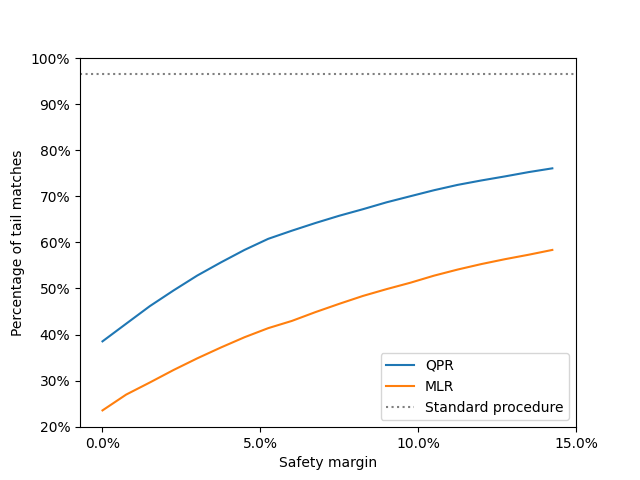
\includegraphics[width=\textwidth]{./project2/figures/tailMatches/regLN.png}
        \caption{Regression metamodels}
    \end{subfigure}\hfill
    \begin{subfigure}{0.48\textwidth}
        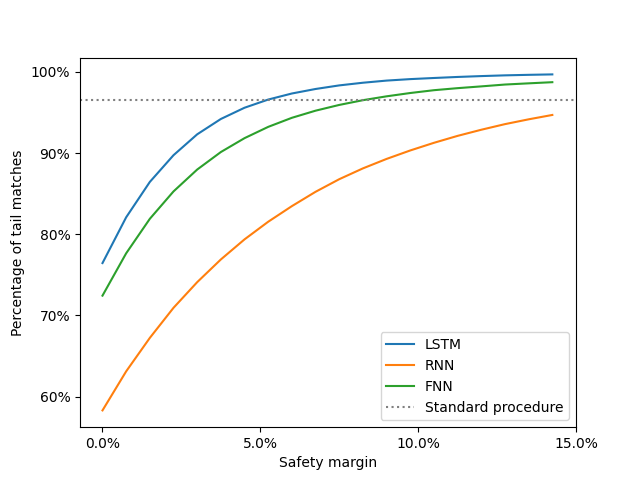
\includegraphics[width=\textwidth]{./project2/figures/tailMatches/nnLN.png}
        \caption{Neural network metamodel}
    \end{subfigure}
    \caption{Percentage of correctly identified true tail scenarios by different metamodels.}
    \label{fig2:tailMatches}
\end{figure}

Figure~\ref{fig2:tailMatches} depicts the average percentage of correctly identified true tail scenarios by different metamodels for increasing safety margins.
Each quantity is averaged over $100$ macro replications.
For a fixed safety margin, the percentage of tail matches of the traditional regression metamodels are substantially lower than the ones of the neural networks.
We observe that a poor metamodel such as the \gls{qpr} identifies less than $40\%$ of the true tail scenario without any safety margin.
In contrast, a well-suited metamodel such as the \gls{lstm} identifies more than $75\%$ of the true tail scenarios without any safety margin and more than the \gls{qpr} metamodel does with $15\%$ of safety margin\footnote{The metamodel in~\cite{dang2020efficient} identifies $100\%$ of the true tail scenarios on with a $10\%$ safety margin for a \gls{gmab} contract.
The \gls{gmab} contract is simpler than the \gls{gmwb} contract, and the true tail scenarios are easier to identify. 
For a \gls{gmab}, our \gls{lstm} metamodel identifies $100\%$ of the true tail scenarios with a $2.5\%$ safety margin}.
The \gls{rnn} metamodel suffers from the vanishing gradient problem during the training stage. 
For some macro replications (as shown in Figure~\ref{subfig2:badRNN}), the \gls{rnn} metamodels' predictions are far from the true losses, especially on the tails.
Seperating the good training macro replications from the bad ones, the results reconcile with the findings in Table~\ref{tab:gmwb_arch}.
The \gls{fnn} metamodel has a better fit than the regression metamodels, but it does not have the same level of accuracy as the \gls{lstm} metamodel, which is a specialized network to capture the sequential structure of our time-series features.
For comparison, the horizontal dotted line shows the percentage of correctly identified true tails for the standard nested simulation procedure.
A good metamodel should be able to identify a similar percentage of true tail scenarios as the standard procedure does with a reasonable safety margin.
Otherwise, the two-stage procedure will offer no computational advantage in simulation budget over the standard procedure.
The \gls{lstm} metamodel can reach similar percentage \textcolor{red}{of correctly identified true tail scenarios} with a $5\%$ safety margin.
This indicates that the \gls{lstm} metamodel should be able to reach the same level of accuracy as the standard procedure with only $20\%$ of the simulation budget.

\begin{figure}[ht!]
    \centering
    \begin{subfigure}{0.48\textwidth}
        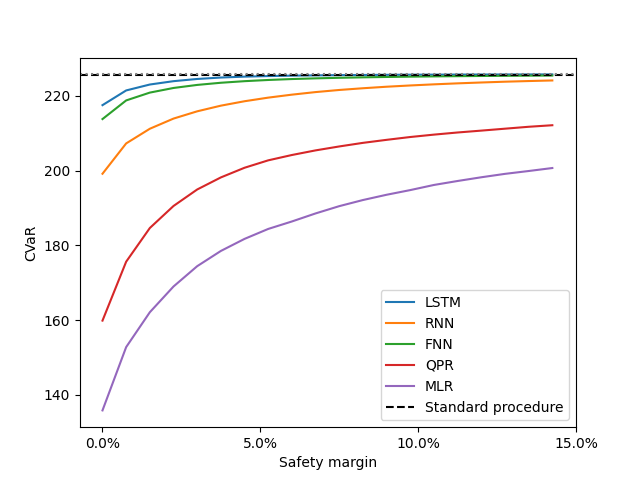
\includegraphics[width=\textwidth]{./project2/figures/CVaR/allLN.png}
        \caption{Safety margin $0\%$ - $15\%$.}
        \label{subfig2:AllSafetyMargin}
    \end{subfigure}
    \begin{subfigure}{0.48\textwidth}
        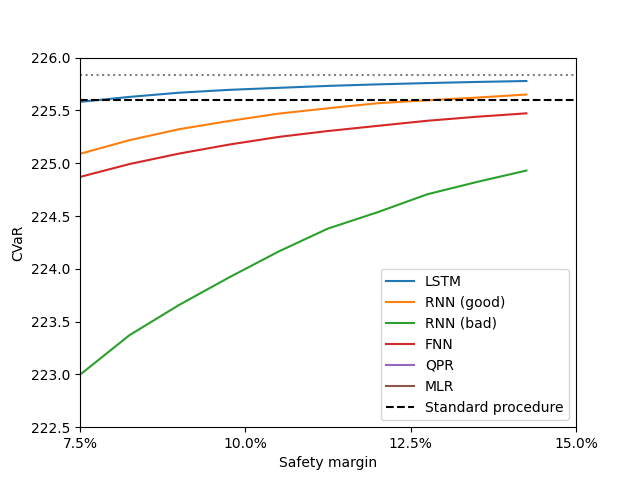
\includegraphics[width=\textwidth]{./project2/figures/CVaR/zoomedLN.png}
        \caption{Safety margin $7.5\%$ - $15\%$.}
        \label{subfig2:ZoomedSafetyMargin}
    \end{subfigure}
    \caption{Average $95\%$-CVaR estimates by different procedures. The right figure is a zoomed-in version of the left figure.} 
    \label{fig2:CVaR95}
\end{figure}

Lastly, we return to our original goal of estimating the $95\%$-\gls{cvar} of the dynamic hedging error.
Figure~\ref{fig2:CVaR95} shows the $95\%$-\gls{cvar} estimates for all five metamodels with different safety margins, averaged over $100$ macro replications.
Figure~\ref{subfig2:ZoomedSafetyMargin} is a zoomed version of Figure~\ref{subfig2:AllSafetyMargin}.
Because the safety margin only affects the two-stage procedure, the true 95\%-\gls{cvar} and the one estimated by the standard procedure are horizontal lines (which are the solid and dotted lines, respectively) in Figure~\ref{fig2:CVaR95}. 
We observe that, with reasonable safety margins, the two-stage procedures with a \gls{lstm} metamodel consistently produce estimates that are as accurate as the standard procedure's estimate.
The amount of computational savings is substantial.
The \gls{lstm} is particularly superior to other metamodels as it accurately identifies the true tail scenarios and produces highly accurate \gls{cvar} estimates with small safety margins.
By concentrating the simulation budget on the predicted tail scenarios, the two-stage procedure with the \gls{lstm} metamodel is able to achieve a similar degree of accuracy as the standard procedure with a much smaller simulation budget.
As the percentage of correctly identified tails approaches $100\%$, the two-stage procedure's \gls{cvar} estimates does not converge to the true \gls{cvar} but to the standard procedure's estimate.
This is because the two-stage procedure's \gls{cvar} estimates are based on the standard procedure's estimates on the predicted tail scenarios, and the standard procedure's estimates themselves are also noisy.

\subsection{Noise Tolerance of DNN Metamodels} \label{subsec2:noiseTolerance}

For financial and actuarial applications, regulators and practitioners are often concerned about the robustness of \gls{dnn} models to noise in training labels, which hinders the adoption of these models in practice.
Since the true relationship is unknown in real-world applications, most deep learning literature illustrates the impact of noise by artificially injecting noise into real-world datasets, which is already noisy prior to the injection.
In our numerical experiments, we are able to use Monte Carlo simulation to generate a true dataset that approximates the true hedging losses with a high degree of precision, and, as a result, we are able to explore the important question of whether deep learning models are indeed capable of learning the true feature-label relationship from noisy training labels.
In this section, we treat the standard nested simulation procedure as a data generator and examine the noise tolerance of \gls{lstm} metamodels by varying the numbers of the outer scenarios ($M$) and the inner replications ($N$) used to generate the training samples.

The number of outer scenarios corresponds to the number of feature-label pairs in the training dataset, and the number of inner replications controls the noise level in the training labels.
Recall that we use the standard nested simulation procedure with $N=100$ inner replications in our previous experiments, and we will refer to the resulting training dataset as the \textit{low-noise dataset}.
We also generate a \textit{medium-noise dataset} and a \textit{high-noise dataset} by running the standard nested simulation procedure with $N=10$ and $N=1$ inner replications, respectively.
By altering the data quantity and quality, we conduct a sensitivity analysis on the \gls{lstm} metamodels' noise tolerance.
We study the impact of noisy data on two \gls{lstm} metamodels with different model capacities, i.e., different numbers of trainable parameters.
The two \gls{lstm} metamodels has the same number of layers, but their numbers of hidden units in each layer are different.
More specfically, the high-capacity \gls{lstm} metamodel has $128$ and $16$ hidden units in the first and second \gls{lstm} layers, respectively, while the low-capacity \gls{lstm} metamodel has $32$ and $4$.

The maximum number of training samples is set to $M = \num{100000}$.
The training samples are split into training and test sets with a $90\%$-$10\%$ split ratio.
The true labels are generated by running the standard nested simulation procedure with $N=\num{100000}$ inner replications for each of the $\num{100000}$ outer scenarios.
The reason for using a maximum of $\num{100000}$ data points is precisely due to the computational cost of running the standard nested simulation procedure.
For consistency, the \gls{lstm} metamodels are trained with the same architecture and training settings as in the previous experiments.

\begin{table}[ht!]
    \small
    \centering
    \begin{tabular}{lccccc}
        \toprule
        \textbf{Model}      & \textbf{$N$}         & \textbf{Training error}                & \textbf{Test error}               & \textbf{True error}\\
        \midrule
        \gls{lstm}                & $\num{100}$                & $0.075 (\pm4.5\times 10^{-3})$         & $0.079(\pm5.4\times 10^{-3})$     & $0.063 (\pm4.4\times 10^{-3})$ \\ 
        High-capacity \gls{lstm}  & $\num{100}$                & $0.068 (\pm3.6\times 10^{-3})$         & $0.102(\pm6.1\times 10^{-2})$     & $0.060 (\pm3.6\times 10^{-3})$ \\
        Average Difference  & $\num{100}$                & $-0.007$                               & $0.023$                           & $-0.003$ \\
        \hline
        \gls{lstm}                & $\num{10}$                 & $0.195 (\pm1.1\times 10^{-3})$         & $0.193(\pm1.7\times 10^{-3})$     & $0.070 (\pm9.1\times 10^{-4})$ \\
        High-capacity \gls{lstm}  & $\num{10}$                 & $0.157 (\pm2.0\times 10^{-3})$         & $0.199(\pm1.9\times 10^{-3})$     & $0.065 (\pm1.9\times 10^{-3})$ \\
        Average Difference  & $\num{10}$                 & $-0.038$                               & $0.006$                           & $-0.005$ \\
        \hline
        \gls{lstm}                & $\num{1}$                  & $1.366 (\pm8.6\times 10^{-3})$         & $0.781(\pm6.0\times 10^{-3})$     & $0.129 (\pm5.0\times 10^{-3})$ \\
        High-capacity \gls{lstm}  & $\num{1}$                  & $1.354 (\pm2.7\times 10^{-2})$         & $0.795(\pm8.3\times10^{-2})$      & $0.149 (\pm2.7\times 10^{-2})$ \\
        Average Difference  & $\num{1}$                  & $-0.012$                               & $0.014$                           & \textcolor{red}{$0.020$} \\
        \bottomrule
    \end{tabular}
    \caption{MSEs of LSTM metamodels.}
    \label{tab:lstm_arch}
\end{table}

The first two rows of Table~\ref{tab:lstm_arch} shows the average squared errors and the half widths of their $95\%$ confidence intervals between the metamodel predictions and the labels in the training dataset and the true dataset.
$N$ indicates the noise level in the training labels, i.e., a simulation dataset with fewer inner replications has a higher noise level.
The test errors are included as a practical measure of the metamodels' generalization ability to unseen noisy samples.
For this particular experiment, we are more interested in the true errors, which measure the metamodels' ability to learn the true feature-label relationship from the low-noise, medium-noise, and high-noise datasets.
We first observe that all the true errors are lower than the training errors, indicating that the \gls{lstm} metamodels generalize well to predicting the true losses.
Both \gls{lstm} metamodels are able to learn the true feature-label relationship from the low-noise and medium-noise datasets.
However, when the noise level is high, both \gls{lstm} metamodels have high true errors.

The differences in the errors between the \gls{lstm} metamodels are also reported in the last rows of Table~\ref{tab:lstm_arch}.
A positive difference indicates that the high-capacity \gls{lstm} has a higher error than the regular \gls{lstm}.
We observe that both \gls{lstm} metamodels have similar errors on the low-noise and medium-noise datasets.
However, when the noise level is high, the high-capacity \gls{lstm} has higher errors than the regular \gls{lstm}.
This is because the high-capacity \gls{lstm} has more trainable parameters and is more prone to over-fitting to the noise in the training labels.
In contrast, the \gls{lstm} metamodel is more robust to label noise and is able to learn the true feature-label relationship better from the high-noise dataset.
In practice, since the true relationship is unknown, the true error is not readily available.
The test error approximates the true error and is directly observable.
The differences in test errors of the \gls{lstm} metamodels are inconsistent with the differences in true errors.
Therefore, test errors are not reliable indicators of the metamodels' noise tolerance.
For practical applications that utilize nerual networks as metamodels, we recommend not to simulate the test scenarios.
Instead, we recommend simulating the true contract losses on a subset of training scenarios to evaluate the metamodels' generalization ability.

In summary, our numerical experiments demonstrate that both \gls{lstm} metamodels are capable of learning the true inner simulation model from the noisy training labels.
In most cases, a high-capacity metamodel is shown to perform better.
Nevertheless, in extreme circumstances when the noise level is too high, using a high capacity metamodel leads to severe over-fitting and poor generalization.
Hence, domain knowledge about the right architecture for the task and knowledge about the noise level in the training labels are beneficial for choosing the correct metamodel.

\begin{figure}[ht!]
    \centering
    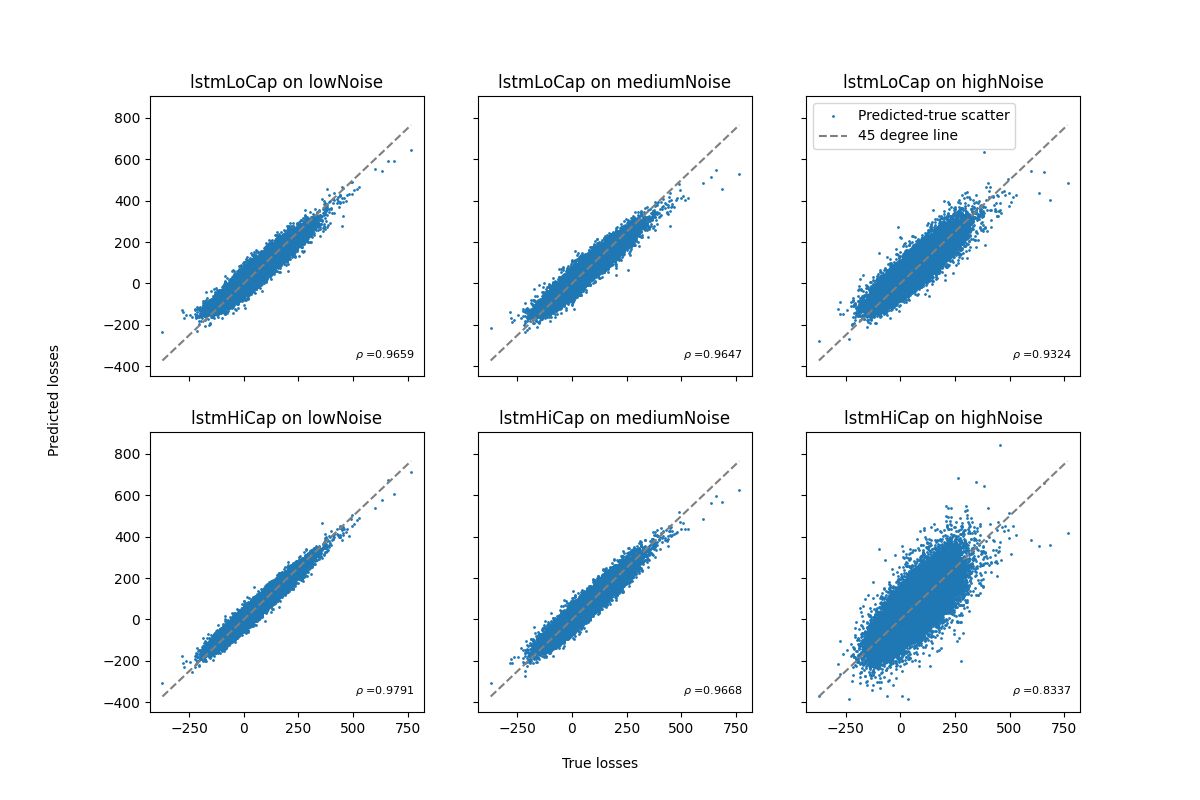
\includegraphics[width=\textwidth]{./project2/figures/qqPlots/lstmAll.png}
    \caption{QQ-plots between true losses (x-axis) and predicted losses (y-axis) for two LSTM metamodels.} 
    \label{fig2:QQ_All}
\end{figure}

In further details, the QQ-plots depicted in Figure~\ref{fig2:QQ_All} illustrates the fit of the two \gls{lstm} metamodels when different noise levels are present in the training labels.
They are arranged in a 2-by-3 grid, where the two rows correspond to the two \gls{lstm} metamodels with different model capacities, and the three columns correspond to the increasing noise levels.
The Pearson correlation coefficient between the true losses and the predicted losses is labeled in each subplot.
The sparsity of the plot increases as we move from left to right, indicating that the noise level in the training labels increases.
There are two key findings.
\begin{enumerate}
    \item   When trained on the low-noise dataset, the metamodel predictions of high-capacity \gls{lstm} align more closely with the true labels than the regular \gls{lstm}.
    This is expected because the high-capacity \gls{lstm} has more trainable parameters and is able to learn more complex relationships better when the noise level is low.
    \item   When the noise level is medium or high, the high-capacity \gls{lstm} is more affected than the regular \gls{lstm}.
    This is because the high-capacity \gls{lstm} has more trainable parameters and is more prone to over-fitting to the noise in the training labels.
    In contrast, the regular \gls{lstm} is more robust to label noise.
\end{enumerate}

To further test the sensitivity of a \gls{lstm} metamodel and provide a more comprehensive view of the noise tolerance of \gls{dnn} models, we conduct a sensitivity analysis on the noise tolerance of the regular \gls{lstm} metamodel by varying the numbers of outer scenarios ($M$) and inner replications ($N$) used to generate the training dataset.
The number of outer scenarios corresponds to the number of data points in the training dataset, and the number of inner replications controls the noise level in the training labels.

\begin{table}[ht!]
    \small
    \centering
    \begin{tabular}{lccccc}
        \toprule
                            & $N=\num{1}$ & $N=\num{10}$  & $N=\num{100}$ & $N=\num{1000}$\\
        \midrule
        $M = \num{100}$      & $1.139$ & $0.229$ & $0.167$ & $0.158$ \\
        $M = \num{1000}$     & $0.559$ & $0.173$ & $0.123$ & $0.127$ \\
        $M = \num{10000}$    & $0.283$ & $0.115$ & $0.099$ & $0.097$ \\
        $M = \num{100000}$   & $0.129$ & $0.070$ & $0.063$ & $0.063$ \\
        \bottomrule
    \end{tabular}
    \caption{MSE between regular LSTM predicted losses and true losses.}
    \label{tab2:lstm_sens}
\end{table}

\begin{table}[ht!]
    \small
    \centering
    \begin{tabular}{lccccc}
        \toprule
                          & $N=\num{1}$ & $N=\num{10}$  & $N=\num{100}$ & $N=\num{1000}$\\
        \midrule
        $M = \num{100}$      & $0.764$ & $0.408$ & $0.131$ & $0.087$ \\
        $M = \num{1000}$     & $0.878$ & $0.367$ & $0.156$ & $0.087$ \\
        $M = \num{10000}$    & $0.351$ & $0.147$ & $0.064$ & $0.063$ \\
        $M = \num{100000}$   & $0.149$ & $0.065$ & $0.060$ & $0.038$ \\
        \bottomrule
    \end{tabular}
    \caption{MSE between high-capacity LSTM predicted losses and true losses.}
    \label{tab2:hicaplstm_sens}
\end{table}

Table~\ref{tab2:lstm_sens} and~\ref{tab2:hicaplstm_sens} show the average squared errors between the \gls{lstm} predictions and the true losses for increasing $M$ and $N$.
The last rows of Table~\ref{tab2:lstm_sens} and Table~\ref{tab2:hicaplstm_sens} show the performance of the regular and high capacity \gls{lstm} metamodels trained with $M=\num{100000}$ training labels with different noise levels.
We observe that an increasing $N$ reduces the \gls{mse}, but the reduction is not substantial for a regular \gls{lstm} when $N$ is larger than $\num{10}$.
For the high-capacity \gls{lstm}, the \gls{mse} is substantially reduced when $N$ is increased from $\num{1}$ to $\num{100}$, but the reduction is not substantial when $N$ is increased from $\num{100}$ to $\num{1000}$.
Another way to interpret the results in Table~\ref{tab2:lstm_sens} is to compare the MSEs for the same budget of $\Gamma = M \times N$. 

Table entries on the same off-diagonal have the same simulation budget $\Gamma$.
For most budgets, the MSEs are also the lowest when $N = 10$.
The results in Table~\ref{tab2:lstm_sens} suggest that the performance of the \gls{lstm} metamodel is more sensitive to the number of outer scenarios than the number of inner replications.
Treating the neural network as an advanced regression metamodel, we find this pheonomenon to be consistent with the results in~\cite{broadie2015risk}, where the authors show that the performance of a regression-based nested simulation procedure is more affected by the number of outer scenarios.
The last row in Table~\ref{tab2:lstm_sens} and ~\ref{tab2:hicaplstm_sens} show that the high-capacity \gls{lstm} metamodel is relatively insensitive to the number of inner replications.
To make the most efficient use of a fixed simulation budget, the number of inner replication should be set constant around $N=10$ while increasing the number of outer scenarios to the maximum.

To further investigate the \gls{lstm} metamodels' sensitivity to data quantity and quality ($M$ and $N$, respectively), we report the Spearman rank correlation coefficients Table~\ref{tab2:lstm_corr}, which measure the ability to rank the scenarios by their true losses.
It is an appropriate measure of the metamodel's performance in the two-stage procedure, where the metamodel is used to identify the predicted tail scenario set, on which extensive simulations are run in stage 2 to estimate the $95\%$-\gls{cvar}.
The Pearson correlation coefficients are also included in the parentheses to illustrate the linear correlation between the predicted losses and the true losses.
They measure the metamodel's overall prediction accuracy.
Our previous numerical experiments illustrated in Figure~\ref{fig2:tailMatches} have shown that the \gls{lstm} metamodel predictions have high \textit{Spearman} correlation with the true labels for the combination $M=\num{100000}$ and $N=\num{100}$.
We intend to examine if \gls{lstm} predictions also have high \textit{Pearson} correlation with the true labels.
A high \textit{Pearson} correlation suggests the possibility of using \gls{lstm} predictions to estimate risk measures directly.

\begin{table}[ht!]
    \small
    \centering
    \begin{tabular}{lccccc}
        \toprule
                           & $N=\num{1}$   & $N=\num{10}$  & $N=\num{100}$ & $N=\num{1000}$ \\
        \midrule
        $M = \num{100}$    & 0.638 (0.881) & 0.875 (0.915) & 0.896 (0.903) & 0.937 (0.941) \\
        $M = \num{1000}$   & 0.722 (0.768) & 0.899 (0.908) & 0.886 (0.891) & 0.922 (0.927) \\
        $M = \num{10000}$  & 0.845 (0.630) & 0.937 (0.900) & 0.908 (0.905) & 0.947 (0.948) \\
        $M = \num{100000}$ & 0.935 (0.640) & 0.963 (0.909) & 0.927 (0.922) & 0.965 (0.966) \\
        \bottomrule
    \end{tabular}
    \caption{Spearman (Pearson) correlation coefficients of high-capacity LSTM predictions.}
    \label{tab2:lstm_corr}
\end{table}

Consistent with our previous numerical experiments, the Spearman correlations of a high-capacity \gls{lstm} is high for a moderate simulation budget. 
For $M= \num{100000}$, the Spearman correlation is relativelyinsensitive to $N$.
This finding supports further budget savings for our two-stage procedure.
In stage 1, we can lower $N$ from $\num{100}$ to $\num{10}$ almost without compromising on tail scenario preditions. 

For an entry of Table~\ref{tab2:lstm_corr}, the total simulation budget $\Gamma = M N$. 
Entries on the same off-diagonal all have the same $\Gamma$.
The Pearson correlation coefficients are substantially lower for $N=\num{1}$ than the other $N$ values.

\begin{figure}
    \centering
    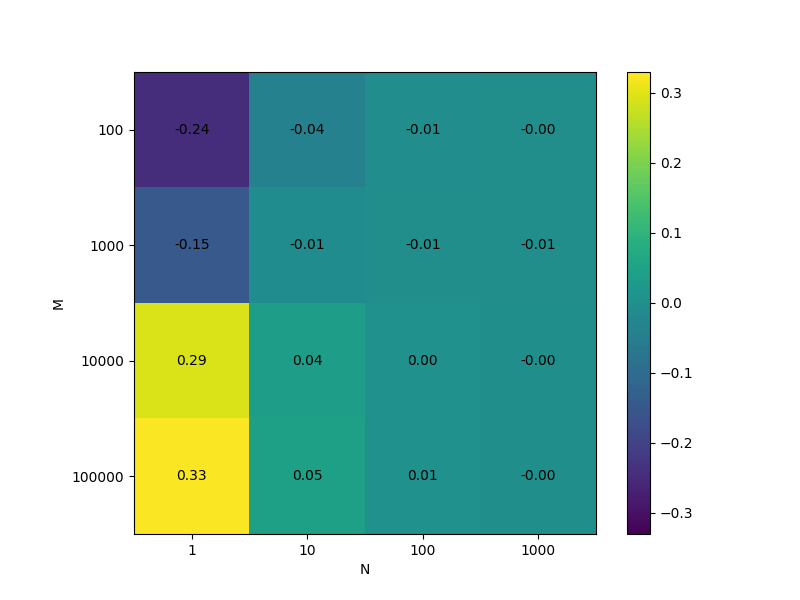
\includegraphics[width=0.6\textwidth]{./project2/figures/cor_heatmap.png}
    \caption{Difference between Spearman and Pearson correlations for high-capacity LSTM metamodel.}
    \label{fig2:cor-heatmap}
\end{figure}

Figure~\ref{fig2:cor-heatmap} shows the difference between the Spearman and Pearson correlation coefficients for the high-capacity \gls{lstm} metamodel.
The heatmap is generated by subtracting the Pearson correlation coefficients from the Spearman correlation.
We observe that Spearman correlation coefficients are not substantially different from the Pearson correlation coefficients for any $N$ larger than $\num{10}$. 
This is a strong evidence that the \gls{lstm} metamodel is not only able to effectively rank the scenarios by their true losses, but also able to make accurate loss predictions.
Instead of using the \gls{lstm} metamodel only for classifying tail scenarios in a two-stage procedure, \gls{lstm}'s ability to cut through a moderate level of noise in training labels encourages us to use its predictions to estimate the \gls{cvar} directly. 

\subsection{Single-Stage Procedure}

The accuracy and robustness of the \gls{lstm} metamodels motivate us to propose a single-stage procedure that uses the metamodel predictions to estimate the \gls{cvar} directly. 
Instead of relying on the standard nested simulation procedure in stage 2, the single-stage procedure can be even more efficient.
In this section, we compare the single-stage procedure to the two-stage procedure and the standard procedure in estimating the $95\%$-\gls{cvar} of the hedging losses for \gls{gmwb}.
In our numerical experiments, the results for the single-stage procedure is obtained with the same metamodels as in the two-stage procedure.
The only difference from Section~\ref{subsec:twoStageProcedure} is that the metamodel predictions are used to estimate the risk measures directly.

\begin{figure}[ht!]
    \centering
    \begin{subfigure}{0.48\textwidth}
        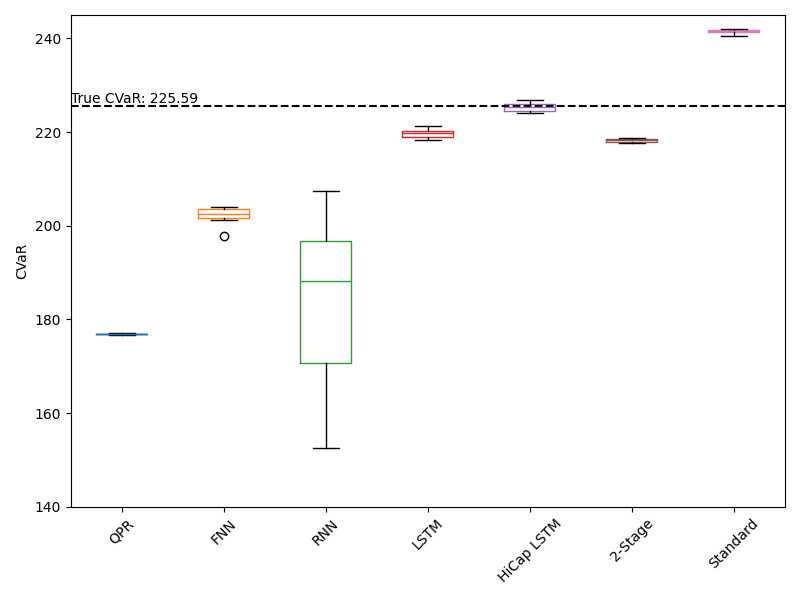
\includegraphics[width=\textwidth]{./project2/figures/singleStage/CVaRmediumNoise.png}
        \caption{Medium noise training labels ($N=10$)}
    \end{subfigure}
    \begin{subfigure}{0.48\textwidth}
        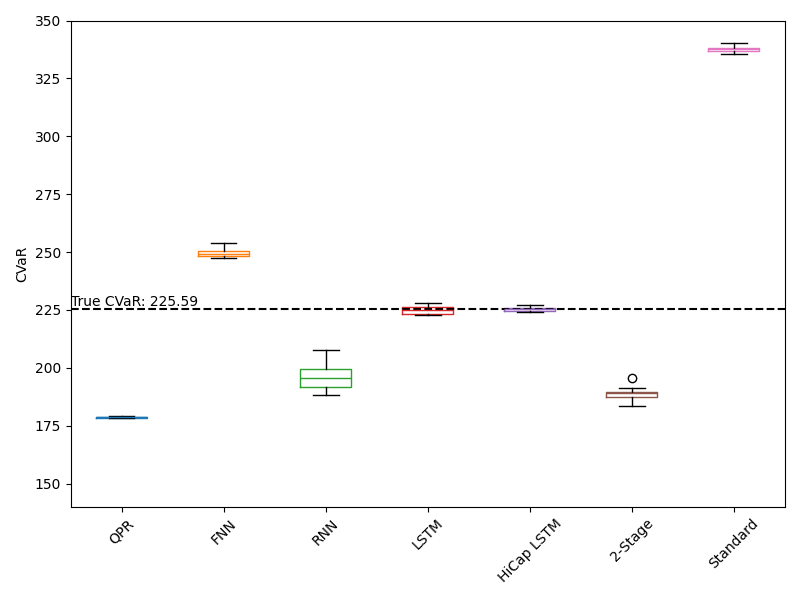
\includegraphics[width=\textwidth]{./project2/figures/singleStage/CVaRhighNoise.png}
        \caption{High noise training labels ($N=1$)}
    \end{subfigure}
    \caption{CVaR estimates of the single-stage procedure with metamodels.}
    \label{fig2:CVaRsingleStage}
\end{figure}

Figure~\ref{fig2:CVaRsingleStage} shows the boxplots of the 95\%-\gls{cvar} estimates of the single-stage procedure with different metamodels and compares them to the two-stage procedure and the standard procedure.
The two-stage procedure uses the same simulation budget as the single-stage procedure in stage 1 with an extra amount of budget for an  extensive inner simulation on the predicted tail scenarios in stage 2.
The metamodel with the best performance in the two-stage procedure is selected, and the safety margin is set to $0\%$.
The standard procedure shown in Figure~\ref{fig2:CVaRsingleStage} uses the noisy loss labels in the training dataset to estimate the \gls{cvar} directly, which uses the same simulation budget as the single-stage procedure.
We observe that the single-stage procedures with the regular \gls{lstm} metamodel consistently produce \gls{cvar} estimates that are closer to the true value than the standard procedure's estimate.
This finding is especially impressive when the noise level in the training labels is high.
It is another strong evidence that a well-selected \gls{lstm} metamodel is able to cut through the noise in the noisy training labels and make accurate loss predictions that lead to accurate \gls{cvar} estimates.
The difference in performance among the metamodels is more pronounced in the single-stage procedure than in the two-stage procedure.
Trained using medium noise labels, the high-capacity \gls{lstm} metamodel consistently produces \gls{cvar} estimates that are closer to the true value than the regular \gls{lstm}, while the other metamodels produce worse estimates.

However, when the noise level in the training labels is high, the high-capacity \gls{lstm} suffers from severe overfitting. 
This is also evident in Table~\ref{tab:lstm_arch}.
Since we are using the metamodel predictions to estimate the \gls{cvar} directly without any safety margin, the metamodel's overall prediction accuracy becomes more important.
In other words, the single-stage procedure is more sensitive to the metamodel's ability to make accurate loss predictions than the two-stage procedure.
Previously, a generic \gls{fnn} metamodel performs well in the two-stage procedure. 
However, results in Figure~\ref{fig2:CVaRsingleStage} suggest that the \gls{fnn} metamodel should not be used in the single-stage procedure.

A single-stage procedure with a regular \gls{lstm} metamodel is particularly superior to the two-stage procedure, as it is able to achieve a higher accuracy as the standard procedure with a much smaller amount of simulation budget.
Note that the single-stage procedure does not require a safety margin.
By avoiding the calibration of the safety margin, it is more straight-forward to implement and is more efficient than the two-stage procedure.
For a two-stage procedure with a $0\%$ safety margin, the extra computational cost is from the extensive inner simulation in stage 2.
On $4$ $20$-core Intel Xeon Gold $\num{6230}$ processors, stage 2 of the two-stage procedure takes $30$ minutes to run with parallel processing, while the $95\%$ confidence band of training time of the high-capacity \gls{lstm} metamodel is $(19.64 \pm 0.94)$ minutes on an Nvidia RTX $\num{3060}$ Ti GPU.
While the accuracy of the two-stage procedure is highly dependent on the safety margin, increasing the safety margin introduces extra computational cost.
Therefore, while achieving a higher accuracy in estimating the \gls{cvar}, the single-stage procedure requires only $60\%$ computation time of the two-stage procedure.

\begin{figure}[ht!]
    \centering
    \begin{subfigure}{0.48\textwidth}
        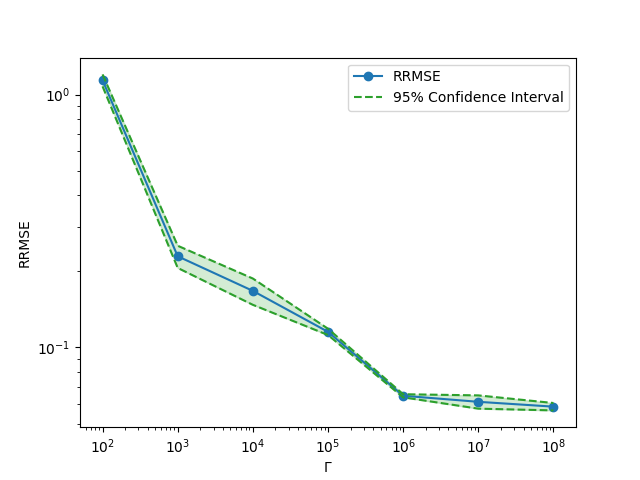
\includegraphics[width=\textwidth]{./project2/figures/singleStage/MSEConvergence_lstmLoCap.png}
        \caption{Regular LSTM}
        \label{subfig2:convLoCap}
    \end{subfigure}
    \begin{subfigure}{0.48\textwidth}
        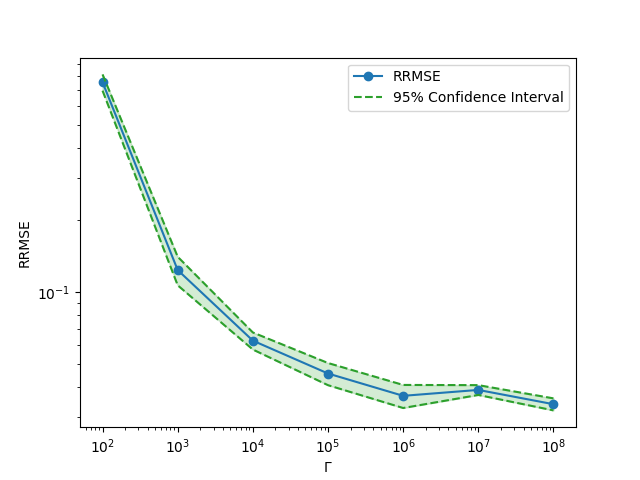
\includegraphics[width=\textwidth]{./project2/figures/singleStage/MSEConvergence_lstmHiCap.png}
        \caption{High-capacity LSTM}
        \label{subfig2:convHiCap}
    \end{subfigure}
    \caption{Empirical convergence of CVaR for the single-stage procedure with LSTM metamodels.} 
    \label{fig2:gammaConvergence}
\end{figure}


To further investigate the single-stage procedure's performance, we conduct a convergence analysis on the \gls{lstm} metamodels.
Figure~\ref{fig2:gammaConvergence} shows the log-log plots of the \gls{rrmse} between the \gls{lstm} metamodel \gls{cvar} predictions and the true \gls{cvar} against the total simulation budget $\Gamma$.
For each budget $\Gamma$, the metamodels are trained for different combinations of $M$ and $N$, and the metamodel with the best \gls{rrmse} is plotted.
While numerical results suggest that the \gls{cvar} estimator of the single-stage procedure with \gls{lstm} metamodels may have better accuracy than the two-stage procedure and the standard procedure when the number of outer scenarios is further increased, we found it difficult to compare their performance due to insufficient computational resources.
For $\Gamma \leq \num{100000}$, the number of outer scenarios is fixed at $M = \num{100000}$, and only the number of inner replications is varied.
Instead, we try to analyze the effect of the number of outer scenarios and the number of inner replications separately by fixing one and varying the other.

\begin{figure}[ht!]
    \centering
    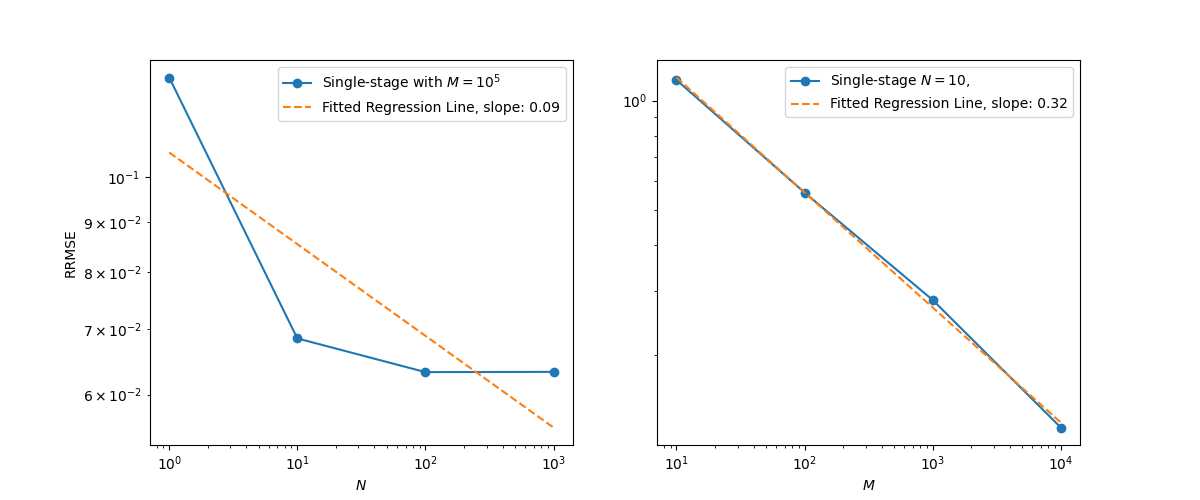
\includegraphics[width=\textwidth]{./project2/figures/singleStage/MSEConvergence_lstmLoCap_MN.png}
    \caption{Empirical convergence of the single-stage procedure with a LSTM metamodel.} 
    \label{fig2:mnConvergence}
\end{figure}

Figure~\ref{fig2:mnConvergence} shows the log-log plots of the \gls{rrmse} between the \gls{lstm} metamodel \gls{cvar} predictions and the true \gls{cvar} against the simulation budget.
The left figure shows the empirical convergence of the \gls{rrmse} for increasing inner replications with a fixed number of outer scenarios ($M=\num{100000}$), and the right figure shows the empirical convergence of the \gls{rrmse} for increasing outer scenarios with a fixed number of inner replications ($N=\num{10}$).
Due to computational constraints, we are not able to run the two-stage procedure and the standard procedure with more outer scenarios or more inner replications, therefore the comparison between the single-stage procedure is only available up to $M = \num{100000}$ and $N = \num{1000}$.
We observe that the \gls{rrmse} decreases as the simulation budget increases, and the rate of convergence is higher when the quantity of the data increases.
For an \gls{lstm} metamodel, increasing the data quality of the training labels has diminishing returns, which is consistent with the results in Figure~\ref{fig2:mnConvergence}.
For an increasing number of inner replications with a fixed number of outer scenarios, the \gls{rrmse} ceases to decrease after reaching $N = \num{100}$. 
More specfically, when the quality of the training labels is fixed at $N = \num{10}$, the \gls{cvar} estimator of a single-stage procedure with a \gls{lstm} metamodel converge roughly in the order of $\mathcal{O}(M^{\frac{2}{3}})$.
This observation resonates with the best possible convergence rate of a standard nested simulation procedure in~\cite{gordy2010nested}.
Hence, in practice, we suggest running the single-stage procedure with a moderate number of inner replications and a large number of outer scenarios to achieve a high level of accuracy with a reasonable computational cost.


\section{Conclusion} \label{sec2:conclusion}
The proposed nested simulation procedures with \gls{dnn} metamodels are shown to result in substantial computational savings in estimating \gls{cvar} of the hedging loss of a \gls{va} contract from accurately predicting the hedging losses and identifying the tail scenarios.
When new outer scenarios are generated, a trained \gls{lstm} metamodel can distinguish between tail and non-tail scenarios and make accurate predictions without the need to run new inner simulations.

Our novel experiment design allows us to examine the impact of label noise on \gls{dnn} models.
We find that a \gls{dnn} with a suitable architecture is able to cut through the noise in training labels and learn the true complex dynamic hedging model.
By showcasing the resilience of these models, our study aims at encouraging regulatory bodies to recognize the value and applicability of deep learning metamodels in financial risk management, and it provides informed suggestions and guidance for the incorporation and oversight of advanced deep learning metamodel in Monte Carlo Simulation in financial applications.
Our findings are particularly insightful in this context.

In our numerical experiments, a \gls{lstm} metamodel is resilient to a high level of noise in training labels and is able to make accurate predictions. 
This is an encouraging evidence that \gls{dnn} metamodels can be used to improve the efficiency of Monte Carlo simulation for quantitative risk management tasks that require a computational-expensive simulation procedure.
We propose two nested simulation procedures that use \gls{dnn} metamodels to estimate risk measures of the hedging loss of a \gls{va} contract.
For estimating tail risk measures, our two-stage procedure is designed to address regulatory concerns by avoiding the direct use of metamodel predictions but instead by using them to identify the potential tail scenarios.
An extensive inner simulation is performed in this chapter to achieve a high level of accuracy on the predicted tail scenarios.
However, the safety margin in the two-stage procedure is a user's choice and is not easy to determine before running extensive numerical experiments.

Our single-stage procedure uses the metamodel predictions to estimate the risk measure directly.
It is more efficient and can be extended to estimate risk measures that require knowledge of the entire loss distribution.
Our numerical experiments demonstrate that the proposed single-stage procedure with \gls{dnn} metamodels result in further computational savings over our two-stage procedure. 
Furthermore, our numerical results provide evidences for adopting \gls{dnn} metamodels in Monte Carlo simulation for risk management tasks.
Through our systematic empirical study of the noise tolerance of \gls{dnn} metamodels, we address regulatory concerns by showing that a \gls{lstm} metamodel with moderate model capacity is resilient to a high level of noise in training labels and is able to make accurate predictions.
A possible future research direction is to apply \gls{dnn} metamodels in other financial risk management tasks that requires complex nested simulation with high-dimensional outer scenarios.
Another future research direction is to investigate the impact of label noise on other deep learning models, such as convolutional neural networks and transformer models, and to compare their performance with \gls{lstm} metamodels in nested simulation procedures. 
From a practical standpoint, the choice of a suitable \gls{dnn} architecture is crucial for the success of a deep learning metamodel in nested simulation procedures.
We find that a \gls{lstm} metamodel is the most suitable for our dynamic hedging simulation model with time series features, but the optimal network architecture may vary for different simulation models.
Exploring \gls{dnn} metamodels in other complex risk management tasks presents a promising avenue for research, especially as these tasks often involve complex, high-dimensional scenarios where traditional methods are insufficient. 
The versatility of neural networks could unlock new insights across a broad spectrum of financial and actuarial applications.

In this chapter, we have demonstrated the potential of \gls{dnn} metamodels to estimate risk measures with high accuracy and efficiency when simulation data is abundant.
In practice, simulation data is often scarce for new market conditions and new insurance products.
\gls{dnn} metamodels are known to suffer from over-fitting when the number of training samples is limited.
In the next chapter, we will extend our study to transfer learning and show that \gls{dnn} metamodels trained on an existing \gls{va} contract can be transferred to a new \gls{va} contract with different market conditions.
We hypothesize that the \gls{dnn} metamodel will generalize well to the new \gls{va} contract, and the computational savings from transfer learning will be substantial.